\documentclass[10pt]{article}
\usepackage[landscape,margin=0.5in]{geometry}
\usepackage{array}
\usepackage{booktabs}
\usepackage{longtable}
\usepackage{amsmath}
\usepackage{graphicx}
\usepackage{float}
\usepackage[T1]{fontenc}
\usepackage{lmodern}
\setlength{\parindent}{0pt}
\setlength{\parskip}{4pt}
\begin{document}

\section*{Sizing the last-30-min straddle trade by the forecast gap: $w_t = f(\mathrm{VRP}_t)$}
\textbf{What is here.} The 15:30 rule trades the straddle (nearest out-of-the-money call and put, same-day expiry, one position) on the sign of $s_t$ = the 16:00-bar variance forecast minus the implied variance at 15:30. This document records every rule that lets the \emph{size} of the position depend on $s_t$ (or on the past distribution of the trade's return given $s_t$), against the flat sign(s) rule on the same days. Two studies, one scorer: the rv\_iv deck's 13-bar recalibration. The proportional and rank rules are scored on the 865 days from the second deck day (the first day has no prior gap to scale by). Each size uses every earlier deck day, back to the first. The Kelly family is a separate sample, the 614 days after a 252-day warm-up. 12 forecasts, midpoint and crossed fills, paired circular block-bootstrap intervals (block 21, 2{,}000 draws). These Sharpes are the deck's and are not comparable with the master table's research-scorer numbers. Every rule is causal: a stake at $t$ uses days before $t$ only (gated by multiplying every future return by 50 and checking that no stake changes). Returns are per unit of premium; the Kelly rules' wealth paths compound.\par
\textbf{Read-offs, recorded from the tables.} Proportional and rank sizing (from the second day): (a) proportional s/rms: 0 of 12 intervals above sign(s), 8 below; (b) rank of $|$s$|$, sign kept: 0 of 12 intervals above sign(s), 0 below; (c) centred rank 2F(s)-1: 0 of 12 intervals above sign(s), 3 below. Kelly family (expanding window, history-ruin-bound cap, every rule $\times$ full/half/quarter): midpoint 0 of 288 rows with an interval above sign(s), 155 below; crossed 0 of 288 above, 170 below.\par
\clearpage
% AUTO-GENERATED by writeup/make_vrp_sizing_tex.py -- do not edit.
\begingroup\scriptsize\setlength{\tabcolsep}{2.5pt}
\begin{longtable}{lrrlrlrl}
\caption{Sizing by the size of the forecast gap, 614 days (after 252-day warm-up), mid fill; the deck's scorer. Every rule keeps the sign of $s$ and changes only the size: (a) proportional, $q_t = s_t / \mathrm{rms}(s)$ with the rms from past days; (b) the rank of $|s_t|$ among past days, sign kept; (c) the centred rank $2F(s_t)-1$. Returns per unit of premium; $\Delta$ = the rule's Sharpe minus sign(s)'s on the same days, with the 95\% interval of a paired circular block bootstrap (block 21, 2{,}000 draws).}\label{tab:vrp_after_252_day_warm_up_mid}\\
\toprule
forecast & sign(s) & \multicolumn{2}{c}{(a) proportional s/rms} & \multicolumn{2}{c}{(b) rank of $|$s$|$, sign kept} & \multicolumn{2}{c}{(c) centred rank 2F(s)-1} \\
 & Sharpe & Sharpe & $\Delta$ vs sign(s) [95\%] & Sharpe & $\Delta$ vs sign(s) [95\%] & Sharpe & $\Delta$ vs sign(s) [95\%] \\
\midrule
\endfirsthead
\caption[]{(continued)}\\
\toprule
forecast & sign(s) & \multicolumn{2}{c}{(a) proportional s/rms} & \multicolumn{2}{c}{(b) rank of $|$s$|$, sign kept} & \multicolumn{2}{c}{(c) centred rank 2F(s)-1} \\
 & Sharpe & Sharpe & $\Delta$ vs sign(s) [95\%] & Sharpe & $\Delta$ vs sign(s) [95\%] & Sharpe & $\Delta$ vs sign(s) [95\%] \\
\midrule
\endhead
\bottomrule
\endlastfoot
baseline (HAR + calendar OLS) & 1.26 & 0.99 & -0.27 [-1.47, +0.92] & 1.29 & +0.03 [-0.71, +0.77] & 0.90 & -0.36 [-1.35, +0.62] \\
block-diagonal ridge & 1.54 & 0.76 & -0.78 [-2.09, +0.62] & 1.58 & +0.04 [-0.73, +0.86] & 1.14 & -0.39 [-1.36, +0.51] \\
block-diagonal ridge, without the FOMC columns & 1.52 & 0.75 & -0.77 [-1.99, +0.59] & 1.64 & +0.13 [-0.59, +0.87] & 1.19 & -0.33 [-1.17, +0.52] \\
LightGBM & 1.44 & 0.73 & -0.70 [-1.88, +1.07] & 1.86 & +0.43 [-0.37, +1.21] & 1.27 & -0.16 [-1.11, +0.80] \\
XGBoost & 1.52 & 0.74 & -0.78 [-2.05, +0.93] & 1.67 & +0.15 [-0.64, +1.06] & 1.14 & -0.38 [-1.50, +0.74] \\
lasso (causally tuned) & 1.86 & 0.88 & -0.98 [-2.22, +0.39] & 1.82 & -0.04 [-0.72, +0.64] & 1.24 & -0.62 [-1.38, +0.22] \\
lasso (fixed 1e-4) & 1.64 & 0.63 & -1.01 [-2.19, +0.25] & 1.54 & -0.10 [-0.74, +0.55] & 1.13 & -0.51 [-1.26, +0.27] \\
elastic net (causally tuned) & 1.28 & 0.77 & -0.51 [-1.91, +0.97] & 1.53 & +0.25 [-0.49, +1.04] & 1.06 & -0.22 [-1.05, +0.63] \\
per-bar ridge (HAR + calendar) & 1.54 & 1.19 & -0.36 [-1.33, +0.65] & 1.53 & -0.01 [-0.63, +0.63] & 1.14 & -0.40 [-1.21, +0.37] \\
per-bar ridge (all features) & 1.46 & 0.73 & -0.73 [-1.86, +0.58] & 1.38 & -0.08 [-0.80, +0.64] & 0.87 & -0.59 [-1.55, +0.31] \\
per-bar lasso (all features) & 1.41 & 0.85 & -0.56 [-1.71, +0.80] & 1.56 & +0.15 [-0.60, +0.92] & 1.10 & -0.31 [-1.29, +0.67] \\
per-bar elastic net (all features) & 1.33 & 0.91 & -0.42 [-1.52, +0.91] & 1.64 & +0.32 [-0.33, +1.02] & 1.18 & -0.15 [-1.03, +0.72] \\
per-bar ridge (live-feasible set) & 1.51 & 0.68 & -0.83 [-2.16, +0.52] & 1.40 & -0.11 [-0.89, +0.62] & 1.04 & -0.47 [-1.41, +0.44] \\
per-bar lasso (live-feasible set) & 1.72 & 1.03 & -0.69 [-1.88, +0.65] & 1.71 & -0.00 [-0.73, +0.71] & 1.39 & -0.33 [-1.34, +0.58] \\
per-bar elastic net (live-feasible set) & 1.76 & 0.83 & -0.93 [-2.10, +0.42] & 1.50 & -0.26 [-1.02, +0.53] & 1.19 & -0.57 [-1.48, +0.33] \\
\end{longtable}
\endgroup

\begingroup\scriptsize\setlength{\tabcolsep}{2.5pt}
\begin{longtable}{lrrlrlrl}
\caption{Sizing by the size of the forecast gap, 614 days (after 252-day warm-up), crossed fill; the deck's scorer. Every rule keeps the sign of $s$ and changes only the size: (a) proportional, $q_t = s_t / \mathrm{rms}(s)$ with the rms from past days; (b) the rank of $|s_t|$ among past days, sign kept; (c) the centred rank $2F(s_t)-1$. Returns per unit of premium; $\Delta$ = the rule's Sharpe minus sign(s)'s on the same days, with the 95\% interval of a paired circular block bootstrap (block 21, 2{,}000 draws).}\label{tab:vrp_after_252_day_warm_up_crossed}\\
\toprule
forecast & sign(s) & \multicolumn{2}{c}{(a) proportional s/rms} & \multicolumn{2}{c}{(b) rank of $|$s$|$, sign kept} & \multicolumn{2}{c}{(c) centred rank 2F(s)-1} \\
 & Sharpe & Sharpe & $\Delta$ vs sign(s) [95\%] & Sharpe & $\Delta$ vs sign(s) [95\%] & Sharpe & $\Delta$ vs sign(s) [95\%] \\
\midrule
\endfirsthead
\caption[]{(continued)}\\
\toprule
forecast & sign(s) & \multicolumn{2}{c}{(a) proportional s/rms} & \multicolumn{2}{c}{(b) rank of $|$s$|$, sign kept} & \multicolumn{2}{c}{(c) centred rank 2F(s)-1} \\
 & Sharpe & Sharpe & $\Delta$ vs sign(s) [95\%] & Sharpe & $\Delta$ vs sign(s) [95\%] & Sharpe & $\Delta$ vs sign(s) [95\%] \\
\midrule
\endhead
\bottomrule
\endlastfoot
baseline (HAR + calendar OLS) & 0.90 & 0.75 & -0.15 [-1.36, +1.07] & 0.93 & +0.04 [-0.69, +0.79] & 0.58 & -0.32 [-1.31, +0.66] \\
block-diagonal ridge & 1.18 & 0.54 & -0.65 [-1.93, +0.75] & 1.22 & +0.04 [-0.74, +0.86] & 0.82 & -0.37 [-1.34, +0.56] \\
block-diagonal ridge, without the FOMC columns & 1.16 & 0.53 & -0.63 [-1.83, +0.72] & 1.29 & +0.12 [-0.59, +0.87] & 0.87 & -0.30 [-1.14, +0.55] \\
LightGBM & 1.07 & 0.57 & -0.50 [-1.69, +1.18] & 1.50 & +0.43 [-0.37, +1.22] & 0.96 & -0.11 [-1.07, +0.84] \\
XGBoost & 1.15 & 0.57 & -0.58 [-1.86, +1.05] & 1.31 & +0.16 [-0.66, +1.07] & 0.82 & -0.33 [-1.46, +0.80] \\
lasso (causally tuned) & 1.50 & 0.65 & -0.85 [-2.09, +0.53] & 1.45 & -0.05 [-0.73, +0.64] & 0.92 & -0.58 [-1.36, +0.27] \\
lasso (fixed 1e-4) & 1.29 & 0.41 & -0.87 [-2.03, +0.39] & 1.18 & -0.11 [-0.77, +0.54] & 0.80 & -0.49 [-1.24, +0.31] \\
elastic net (causally tuned) & 0.92 & 0.55 & -0.37 [-1.76, +1.09] & 1.17 & +0.25 [-0.48, +1.05] & 0.75 & -0.17 [-1.01, +0.68] \\
per-bar ridge (HAR + calendar) & 1.18 & 0.96 & -0.22 [-1.24, +0.78] & 1.18 & -0.00 [-0.61, +0.64] & 0.81 & -0.37 [-1.18, +0.41] \\
per-bar ridge (all features) & 1.10 & 0.50 & -0.60 [-1.72, +0.71] & 1.03 & -0.07 [-0.78, +0.64] & 0.55 & -0.54 [-1.52, +0.37] \\
per-bar lasso (all features) & 1.05 & 0.61 & -0.44 [-1.58, +0.90] & 1.19 & +0.14 [-0.63, +0.92] & 0.76 & -0.29 [-1.28, +0.72] \\
per-bar elastic net (all features) & 0.96 & 0.67 & -0.30 [-1.40, +1.01] & 1.27 & +0.31 [-0.34, +1.01] & 0.84 & -0.12 [-1.00, +0.76] \\
per-bar ridge (live-feasible set) & 1.15 & 0.45 & -0.70 [-2.05, +0.66] & 1.04 & -0.11 [-0.90, +0.63] & 0.71 & -0.44 [-1.41, +0.47] \\
per-bar lasso (live-feasible set) & 1.36 & 0.79 & -0.56 [-1.75, +0.77] & 1.35 & -0.00 [-0.72, +0.72] & 1.06 & -0.30 [-1.31, +0.62] \\
per-bar elastic net (live-feasible set) & 1.40 & 0.60 & -0.80 [-1.98, +0.53] & 1.14 & -0.26 [-1.02, +0.55] & 0.85 & -0.55 [-1.47, +0.38] \\
\end{longtable}
\endgroup

\begingroup\scriptsize\setlength{\tabcolsep}{2.5pt}
\begin{longtable}{lrrlrlrl}
\caption{Sizing by the size of the forecast gap, 865 days (from the second day), mid fill; the deck's scorer. Every rule keeps the sign of $s$ and changes only the size: (a) proportional, $q_t = s_t / \mathrm{rms}(s)$ with the rms from past days; (b) the rank of $|s_t|$ among past days, sign kept; (c) the centred rank $2F(s_t)-1$. Returns per unit of premium; $\Delta$ = the rule's Sharpe minus sign(s)'s on the same days, with the 95\% interval of a paired circular block bootstrap (block 21, 2{,}000 draws).}\label{tab:vrp_from_the_second_day_mid}\\
\toprule
forecast & sign(s) & \multicolumn{2}{c}{(a) proportional s/rms} & \multicolumn{2}{c}{(b) rank of $|$s$|$, sign kept} & \multicolumn{2}{c}{(c) centred rank 2F(s)-1} \\
 & Sharpe & Sharpe & $\Delta$ vs sign(s) [95\%] & Sharpe & $\Delta$ vs sign(s) [95\%] & Sharpe & $\Delta$ vs sign(s) [95\%] \\
\midrule
\endfirsthead
\caption[]{(continued)}\\
\toprule
forecast & sign(s) & \multicolumn{2}{c}{(a) proportional s/rms} & \multicolumn{2}{c}{(b) rank of $|$s$|$, sign kept} & \multicolumn{2}{c}{(c) centred rank 2F(s)-1} \\
 & Sharpe & Sharpe & $\Delta$ vs sign(s) [95\%] & Sharpe & $\Delta$ vs sign(s) [95\%] & Sharpe & $\Delta$ vs sign(s) [95\%] \\
\midrule
\endhead
\bottomrule
\endlastfoot
baseline (HAR + calendar OLS) & 0.98 & -0.44 & -1.42 [-2.38, +0.28] & 0.98 & -0.01 [-0.66, +0.63] & 0.69 & -0.29 [-1.02, +0.42] \\
block-diagonal ridge & 1.36 & -0.70 & -2.05 [-3.05, -0.26] & 1.13 & -0.23 [-0.90, +0.49] & 0.62 & -0.74 [-1.52, +0.14] \\
block-diagonal ridge, without the FOMC columns & 1.29 & -0.70 & -1.98 [-2.96, -0.31] & 1.14 & -0.15 [-0.73, +0.48] & 0.62 & -0.67 [-1.40, +0.11] \\
LightGBM & 1.48 & -0.36 & -1.84 [-2.84, +0.01] & 1.53 & +0.06 [-0.60, +0.72] & 1.18 & -0.29 [-1.07, +0.43] \\
XGBoost & 1.52 & 0.03 & -1.49 [-2.46, +0.06] & 1.55 & +0.04 [-0.59, +0.69] & 1.23 & -0.28 [-1.11, +0.53] \\
lasso (causally tuned) & 1.43 & -0.65 & -2.08 [-3.04, -0.41] & 1.30 & -0.13 [-0.73, +0.51] & 0.65 & -0.78 [-1.48, -0.02] \\
lasso (fixed 1e-4) & 1.53 & -0.70 & -2.23 [-3.14, -0.66] & 1.08 & -0.45 [-1.06, +0.22] & 0.57 & -0.96 [-1.82, -0.09] \\
elastic net (causally tuned) & 1.04 & -0.63 & -1.67 [-2.58, -0.16] & 0.94 & -0.10 [-0.65, +0.51] & 0.50 & -0.54 [-1.19, +0.16] \\
per-bar ridge (HAR + calendar) & 1.27 & -0.48 & -1.75 [-2.65, +0.03] & 1.26 & -0.01 [-0.56, +0.54] & 0.92 & -0.35 [-1.01, +0.30] \\
per-bar ridge (all features) & 1.79 & -0.00 & -1.80 [-2.68, -0.61] & 1.34 & -0.45 [-1.06, +0.16] & 0.64 & -1.15 [-2.03, -0.31] \\
per-bar lasso (all features) & 1.46 & -0.36 & -1.82 [-2.65, -0.33] & 1.37 & -0.09 [-0.72, +0.57] & 0.99 & -0.47 [-1.19, +0.26] \\
per-bar elastic net (all features) & 1.59 & -0.24 & -1.83 [-2.67, -0.44] & 1.49 & -0.10 [-0.69, +0.53] & 1.10 & -0.49 [-1.14, +0.20] \\
per-bar ridge (live-feasible set) & 1.70 & -0.40 & -2.10 [-3.17, -0.58] & 1.30 & -0.40 [-0.97, +0.22] & 0.72 & -0.98 [-1.87, -0.10] \\
per-bar lasso (live-feasible set) & 1.59 & -0.52 & -2.12 [-3.04, -0.43] & 1.35 & -0.24 [-0.85, +0.37] & 1.07 & -0.52 [-1.19, +0.15] \\
per-bar elastic net (live-feasible set) & 1.72 & -0.49 & -2.21 [-3.14, -0.63] & 1.33 & -0.38 [-0.97, +0.22] & 1.05 & -0.67 [-1.31, -0.01] \\
\end{longtable}
\endgroup

\begingroup\scriptsize\setlength{\tabcolsep}{2.5pt}
\begin{longtable}{lrrlrlrl}
\caption{Sizing by the size of the forecast gap, 865 days (from the second day), crossed fill; the deck's scorer. Every rule keeps the sign of $s$ and changes only the size: (a) proportional, $q_t = s_t / \mathrm{rms}(s)$ with the rms from past days; (b) the rank of $|s_t|$ among past days, sign kept; (c) the centred rank $2F(s_t)-1$. Returns per unit of premium; $\Delta$ = the rule's Sharpe minus sign(s)'s on the same days, with the 95\% interval of a paired circular block bootstrap (block 21, 2{,}000 draws).}\label{tab:vrp_from_the_second_day_crossed}\\
\toprule
forecast & sign(s) & \multicolumn{2}{c}{(a) proportional s/rms} & \multicolumn{2}{c}{(b) rank of $|$s$|$, sign kept} & \multicolumn{2}{c}{(c) centred rank 2F(s)-1} \\
 & Sharpe & Sharpe & $\Delta$ vs sign(s) [95\%] & Sharpe & $\Delta$ vs sign(s) [95\%] & Sharpe & $\Delta$ vs sign(s) [95\%] \\
\midrule
\endfirsthead
\caption[]{(continued)}\\
\toprule
forecast & sign(s) & \multicolumn{2}{c}{(a) proportional s/rms} & \multicolumn{2}{c}{(b) rank of $|$s$|$, sign kept} & \multicolumn{2}{c}{(c) centred rank 2F(s)-1} \\
 & Sharpe & Sharpe & $\Delta$ vs sign(s) [95\%] & Sharpe & $\Delta$ vs sign(s) [95\%] & Sharpe & $\Delta$ vs sign(s) [95\%] \\
\midrule
\endhead
\bottomrule
\endlastfoot
baseline (HAR + calendar OLS) & 0.51 & -0.54 & -1.04 [-1.97, +0.57] & 0.50 & -0.00 [-0.69, +0.65] & 0.24 & -0.27 [-0.99, +0.44] \\
block-diagonal ridge & 0.89 & -0.77 & -1.65 [-2.63, -0.07] & 0.64 & -0.25 [-0.93, +0.49] & 0.18 & -0.70 [-1.47, +0.17] \\
block-diagonal ridge, without the FOMC columns & 0.82 & -0.77 & -1.59 [-2.56, -0.07] & 0.66 & -0.16 [-0.78, +0.50] & 0.19 & -0.63 [-1.35, +0.14] \\
LightGBM & 1.00 & -0.48 & -1.48 [-2.47, +0.21] & 1.08 & +0.08 [-0.65, +0.76] & 0.77 & -0.23 [-1.03, +0.50] \\
XGBoost & 1.04 & -0.17 & -1.21 [-2.17, +0.33] & 1.10 & +0.07 [-0.61, +0.75] & 0.81 & -0.23 [-1.06, +0.59] \\
lasso (causally tuned) & 0.95 & -0.71 & -1.66 [-2.62, -0.18] & 0.80 & -0.16 [-0.78, +0.49] & 0.22 & -0.73 [-1.43, +0.03] \\
lasso (fixed 1e-4) & 1.06 & -0.76 & -1.83 [-2.76, -0.42] & 0.59 & -0.47 [-1.11, +0.23] & 0.13 & -0.93 [-1.77, -0.07] \\
elastic net (causally tuned) & 0.56 & -0.69 & -1.25 [-2.17, +0.11] & 0.44 & -0.12 [-0.67, +0.50] & 0.07 & -0.49 [-1.13, +0.20] \\
per-bar ridge (HAR + calendar) & 0.79 & -0.56 & -1.35 [-2.26, +0.28] & 0.79 & -0.01 [-0.57, +0.56] & 0.46 & -0.33 [-0.99, +0.33] \\
per-bar ridge (all features) & 1.32 & -0.18 & -1.50 [-2.41, -0.32] & 0.85 & -0.48 [-1.11, +0.15] & 0.22 & -1.11 [-1.98, -0.26] \\
per-bar lasso (all features) & 0.99 & -0.45 & -1.44 [-2.30, -0.06] & 0.87 & -0.12 [-0.77, +0.56] & 0.52 & -0.47 [-1.19, +0.27] \\
per-bar elastic net (all features) & 1.13 & -0.35 & -1.48 [-2.33, -0.16] & 1.00 & -0.13 [-0.71, +0.52] & 0.64 & -0.49 [-1.15, +0.21] \\
per-bar ridge (live-feasible set) & 1.23 & -0.52 & -1.75 [-2.85, -0.28] & 0.81 & -0.42 [-1.00, +0.22] & 0.28 & -0.95 [-1.83, -0.07] \\
per-bar lasso (live-feasible set) & 1.12 & -0.61 & -1.73 [-2.66, -0.22] & 0.86 & -0.26 [-0.89, +0.38] & 0.61 & -0.52 [-1.21, +0.18] \\
per-bar elastic net (live-feasible set) & 1.25 & -0.58 & -1.83 [-2.77, -0.38] & 0.85 & -0.40 [-1.01, +0.25] & 0.59 & -0.66 [-1.33, +0.02] \\
\end{longtable}
\endgroup

\begingroup\scriptsize\setlength{\tabcolsep}{2.5pt}
\begin{longtable}{lrlrrrr}
\caption{Kelly-type sizing, 614 days after the 252-day warm-up, mid fill; the deck's scorer; expanding estimation window, stake capped at the history ruin bound $1/|\min_{u<t} R'_u|$. Rules (every quantity at $t$ from days before $t$): (a) Kelly $f=\hat\mu/\hat\sigma^2$ with the mean and variance of the trade's return conditional on $|s|$ terciles $\times$ sign, or on a regression of the return on $(s, |s|)$ with or without a sign intercept; (b) Kelly by the sign of $s$ alone (log-optimal, and mean--variance); (c) proportional to $s$ at the sign(s) Kelly stake; (d) always short at its Kelly stake; and sign(s) itself levered at its Kelly stake. Fractions full / half / quarter. $g$ = annualized mean of $\log(1 + w_t R'_t)$; max DD = the largest fall of wealth from its running peak; mean $|w|$ = the average stake as a share of wealth; opposite side = share of days the rule takes the side opposite to sign(s). $\Delta$ = the rule's Sharpe minus sign(s)'s with the paired 95\% interval (block 21, 2{,}000 draws).}\label{tab:kelly_mid}\\
\toprule
rule (Kelly fraction) & Sharpe & $\Delta$Sharpe vs sign(s) [95\%] & growth $g$ & max DD & mean $|w|$ & opposite side \% \\
\midrule
\endfirsthead
\caption[]{(continued)}\\
\toprule
rule (Kelly fraction) & Sharpe & $\Delta$Sharpe vs sign(s) [95\%] & growth $g$ & max DD & mean $|w|$ & opposite side \% \\
\midrule
\endhead
\bottomrule
\endlastfoot
\multicolumn{7}{l}{\quad\emph{baseline (HAR + calendar OLS)}: sign(s), one unit of premium, Sharpe 1.26, growth at 3\% of wealth 0.54} \\
(c) proportional s/rms (unit, x10) & 0.99 & -0.27 [-1.47, +0.92] & 0.07 & -0.06 & 0.10 & 0 \\
(d) always short, Kelly (full) & -0.16 & -1.42 [-2.69, -0.17] & -0.15 & -0.55 & 0.02 & 26 \\
(d) always short, Kelly (half) & -0.16 & -1.42 [-2.69, -0.17] & -0.05 & -0.31 & 0.01 & 26 \\
(d) always short, Kelly (quarter) & -0.16 & -1.42 [-2.69, -0.17] & -0.02 & -0.16 & 0.00 & 26 \\
sign(s), Kelly-levered (full) & 0.90 & -0.36 [-0.84, +0.13] & 0.39 & -0.57 & 0.04 & 0 \\
sign(s), Kelly-levered (half) & 0.90 & -0.36 [-0.84, +0.13] & 0.29 & -0.33 & 0.02 & 0 \\
sign(s), Kelly-levered (quarter) & 0.90 & -0.36 [-0.84, +0.13] & 0.17 & -0.17 & 0.01 & 0 \\
(b) Kelly by sign of s, log-optimal (full) & 0.57 & -0.69 [-1.35, -0.03] & 0.08 & -0.58 & 0.04 & 13 \\
(b) Kelly by sign of s, log-optimal (half) & 0.57 & -0.69 [-1.35, -0.03] & 0.15 & -0.32 & 0.02 & 13 \\
(b) Kelly by sign of s, log-optimal (quarter) & 0.57 & -0.69 [-1.35, -0.03] & 0.10 & -0.17 & 0.01 & 13 \\
(b') Kelly by sign of s, mean-variance (full) & 0.57 & -0.69 [-1.35, -0.01] & 0.05 & -0.62 & 0.04 & 13 \\
(b') Kelly by sign of s, mean-variance (half) & 0.57 & -0.69 [-1.35, -0.01] & 0.15 & -0.35 & 0.02 & 13 \\
(b') Kelly by sign of s, mean-variance (quarter) & 0.57 & -0.69 [-1.35, -0.01] & 0.11 & -0.18 & 0.01 & 13 \\
(a) Kelly by sign x $|$s$|$ 3 bins (full) & -0.74 & -2.00 [-3.13, -0.91] & -1.34 & -0.97 & 0.05 & 30 \\
(a) Kelly by sign x $|$s$|$ 3 bins (half) & -0.23 & -1.50 [-2.70, -0.21] & -0.46 & -0.84 & 0.03 & 30 \\
(a) Kelly by sign x $|$s$|$ 3 bins (quarter) & -0.22 & -1.48 [-2.67, -0.18] & -0.19 & -0.62 & 0.02 & 30 \\
(a) Kelly by regression on s, $|$s$|$ (full) & -0.25 & -1.52 [-2.86, -0.29] & -0.36 & -0.60 & 0.03 & 51 \\
(a) Kelly by regression on s, $|$s$|$ (half) & -0.25 & -1.52 [-2.86, -0.29] & -0.13 & -0.32 & 0.01 & 51 \\
(a) Kelly by regression on s, $|$s$|$ (quarter) & -0.25 & -1.52 [-2.86, -0.29] & -0.05 & -0.17 & 0.01 & 51 \\
(a) Kelly by regression on sign(s), s, $|$s$|$ (full) & 0.70 & -0.56 [-1.11, +0.02] & 0.05 & -0.70 & 0.06 & 6 \\
(a) Kelly by regression on sign(s), s, $|$s$|$ (half) & 0.65 & -0.62 [-1.17, -0.02] & 0.20 & -0.42 & 0.03 & 6 \\
(a) Kelly by regression on sign(s), s, $|$s$|$ (quarter) & 0.65 & -0.62 [-1.17, -0.02] & 0.15 & -0.22 & 0.01 & 6 \\
(c) proportional s/mean$|$s$|$, sign(s) Kelly stake (full) & 1.15 & -0.11 [-1.29, +1.11] & 0.31 & -0.23 & 0.01 & 0 \\
(c) proportional s/mean$|$s$|$, sign(s) Kelly stake (half) & 1.03 & -0.23 [-1.41, +1.05] & 0.16 & -0.13 & 0.01 & 0 \\
(c) proportional s/mean$|$s$|$, sign(s) Kelly stake (quarter) & 0.96 & -0.31 [-1.50, +0.99] & 0.08 & -0.07 & 0.00 & 0 \\
\multicolumn{7}{l}{\quad\emph{block-diagonal ridge}: sign(s), one unit of premium, Sharpe 1.54, growth at 3\% of wealth 0.69} \\
(c) proportional s/rms (unit, x10) & 0.76 & -0.78 [-2.09, +0.62] & 0.06 & -0.11 & 0.11 & 0 \\
(d) always short, Kelly (full) & -0.16 & -1.70 [-3.23, -0.11] & -0.15 & -0.55 & 0.02 & 33 \\
(d) always short, Kelly (half) & -0.16 & -1.70 [-3.23, -0.11] & -0.05 & -0.31 & 0.01 & 33 \\
(d) always short, Kelly (quarter) & -0.16 & -1.70 [-3.23, -0.11] & -0.02 & -0.16 & 0.00 & 33 \\
sign(s), Kelly-levered (full) & 1.35 & -0.19 [-0.40, +0.04] & 0.89 & -0.74 & 0.06 & 0 \\
sign(s), Kelly-levered (half) & 1.35 & -0.19 [-0.40, +0.04] & 0.62 & -0.43 & 0.03 & 0 \\
sign(s), Kelly-levered (quarter) & 1.35 & -0.19 [-0.40, +0.04] & 0.35 & -0.23 & 0.02 & 0 \\
(b) Kelly by sign of s, log-optimal (full) & 1.18 & -0.36 [-0.71, +0.03] & 0.66 & -0.76 & 0.06 & 0 \\
(b) Kelly by sign of s, log-optimal (half) & 1.16 & -0.38 [-0.74, +0.03] & 0.50 & -0.46 & 0.03 & 0 \\
(b) Kelly by sign of s, log-optimal (quarter) & 1.16 & -0.38 [-0.74, +0.03] & 0.30 & -0.24 & 0.02 & 0 \\
(b') Kelly by sign of s, mean-variance (full) & 1.28 & -0.26 [-0.62, +0.19] & 0.75 & -0.75 & 0.06 & 0 \\
(b') Kelly by sign of s, mean-variance (half) & 1.18 & -0.35 [-0.79, +0.18] & 0.53 & -0.50 & 0.03 & 0 \\
(b') Kelly by sign of s, mean-variance (quarter) & 1.18 & -0.35 [-0.79, +0.18] & 0.32 & -0.26 & 0.02 & 0 \\
(a) Kelly by sign x $|$s$|$ 3 bins (full) & -0.01 & -1.55 [-2.45, -0.72] & -0.97 & -0.96 & 0.07 & 24 \\
(a) Kelly by sign x $|$s$|$ 3 bins (half) & 0.06 & -1.48 [-2.35, -0.59] & -0.38 & -0.87 & 0.04 & 24 \\
(a) Kelly by sign x $|$s$|$ 3 bins (quarter) & -0.15 & -1.69 [-2.56, -0.71] & -0.26 & -0.73 & 0.02 & 24 \\
(a) Kelly by regression on s, $|$s$|$ (full) & -0.18 & -1.72 [-3.18, -0.19] & -0.40 & -0.71 & 0.03 & 61 \\
(a) Kelly by regression on s, $|$s$|$ (half) & -0.18 & -1.72 [-3.18, -0.19] & -0.13 & -0.41 & 0.02 & 61 \\
(a) Kelly by regression on s, $|$s$|$ (quarter) & -0.18 & -1.72 [-3.18, -0.19] & -0.05 & -0.22 & 0.01 & 61 \\
(a) Kelly by regression on sign(s), s, $|$s$|$ (full) & 1.34 & -0.19 [-0.60, +0.22] & 0.88 & -0.78 & 0.08 & 4 \\
(a) Kelly by regression on sign(s), s, $|$s$|$ (half) & 1.22 & -0.32 [-0.78, +0.27] & 0.65 & -0.65 & 0.04 & 4 \\
(a) Kelly by regression on sign(s), s, $|$s$|$ (quarter) & 1.22 & -0.32 [-0.78, +0.27] & 0.43 & -0.35 & 0.02 & 4 \\
(c) proportional s/mean$|$s$|$, sign(s) Kelly stake (full) & 0.73 & -0.81 [-2.15, +0.77] & 0.22 & -0.63 & 0.02 & 0 \\
(c) proportional s/mean$|$s$|$, sign(s) Kelly stake (half) & 0.80 & -0.74 [-2.04, +0.74] & 0.18 & -0.35 & 0.01 & 0 \\
(c) proportional s/mean$|$s$|$, sign(s) Kelly stake (quarter) & 0.74 & -0.80 [-2.09, +0.63] & 0.10 & -0.18 & 0.01 & 0 \\
\multicolumn{7}{l}{\quad\emph{block-diagonal ridge, without the FOMC columns}: sign(s), one unit of premium, Sharpe 1.52, growth at 3\% of wealth 0.67} \\
(c) proportional s/rms (unit, x10) & 0.75 & -0.77 [-1.99, +0.59] & 0.06 & -0.11 & 0.11 & 0 \\
(d) always short, Kelly (full) & -0.16 & -1.68 [-3.25, -0.06] & -0.15 & -0.55 & 0.02 & 35 \\
(d) always short, Kelly (half) & -0.16 & -1.68 [-3.25, -0.06] & -0.05 & -0.31 & 0.01 & 35 \\
(d) always short, Kelly (quarter) & -0.16 & -1.68 [-3.25, -0.06] & -0.02 & -0.16 & 0.00 & 35 \\
sign(s), Kelly-levered (full) & 1.32 & -0.20 [-0.65, +0.25] & 0.81 & -0.68 & 0.05 & 0 \\
sign(s), Kelly-levered (half) & 1.32 & -0.20 [-0.65, +0.25] & 0.53 & -0.38 & 0.03 & 0 \\
sign(s), Kelly-levered (quarter) & 1.32 & -0.20 [-0.65, +0.25] & 0.30 & -0.20 & 0.01 & 0 \\
(b) Kelly by sign of s, log-optimal (full) & 1.14 & -0.37 [-0.97, +0.27] & 0.58 & -0.71 & 0.05 & 4 \\
(b) Kelly by sign of s, log-optimal (half) & 1.11 & -0.41 [-1.02, +0.27] & 0.42 & -0.40 & 0.02 & 4 \\
(b) Kelly by sign of s, log-optimal (quarter) & 1.11 & -0.41 [-1.02, +0.27] & 0.24 & -0.20 & 0.01 & 4 \\
(b') Kelly by sign of s, mean-variance (full) & 1.22 & -0.29 [-0.90, +0.39] & 0.65 & -0.70 & 0.05 & 4 \\
(b') Kelly by sign of s, mean-variance (half) & 1.12 & -0.40 [-1.05, +0.37] & 0.44 & -0.44 & 0.02 & 4 \\
(b') Kelly by sign of s, mean-variance (quarter) & 1.12 & -0.40 [-1.05, +0.37] & 0.26 & -0.22 & 0.01 & 4 \\
(a) Kelly by sign x $|$s$|$ 3 bins (full) & -0.04 & -1.56 [-2.66, -0.44] & -0.78 & -0.94 & 0.06 & 30 \\
(a) Kelly by sign x $|$s$|$ 3 bins (half) & 0.17 & -1.35 [-2.44, -0.21] & -0.21 & -0.81 & 0.04 & 30 \\
(a) Kelly by sign x $|$s$|$ 3 bins (quarter) & 0.21 & -1.31 [-2.36, -0.14] & -0.03 & -0.55 & 0.02 & 30 \\
(a) Kelly by regression on s, $|$s$|$ (full) & -0.13 & -1.65 [-3.20, -0.11] & -0.35 & -0.68 & 0.03 & 63 \\
(a) Kelly by regression on s, $|$s$|$ (half) & -0.13 & -1.65 [-3.20, -0.11] & -0.11 & -0.39 & 0.02 & 63 \\
(a) Kelly by regression on s, $|$s$|$ (quarter) & -0.13 & -1.65 [-3.20, -0.11] & -0.04 & -0.21 & 0.01 & 63 \\
(a) Kelly by regression on sign(s), s, $|$s$|$ (full) & 1.28 & -0.23 [-0.72, +0.31] & 0.76 & -0.74 & 0.07 & 5 \\
(a) Kelly by regression on sign(s), s, $|$s$|$ (half) & 1.16 & -0.35 [-0.90, +0.35] & 0.57 & -0.59 & 0.04 & 5 \\
(a) Kelly by regression on sign(s), s, $|$s$|$ (quarter) & 1.16 & -0.35 [-0.90, +0.35] & 0.37 & -0.30 & 0.02 & 5 \\
(c) proportional s/mean$|$s$|$, sign(s) Kelly stake (full) & 0.95 & -0.57 [-1.80, +0.89] & 0.29 & -0.45 & 0.02 & 0 \\
(c) proportional s/mean$|$s$|$, sign(s) Kelly stake (half) & 0.90 & -0.61 [-1.83, +0.79] & 0.17 & -0.23 & 0.01 & 0 \\
(c) proportional s/mean$|$s$|$, sign(s) Kelly stake (quarter) & 0.88 & -0.64 [-1.85, +0.76] & 0.09 & -0.12 & 0.00 & 0 \\
\multicolumn{7}{l}{\quad\emph{LightGBM}: sign(s), one unit of premium, Sharpe 1.44, growth at 3\% of wealth 0.63} \\
(c) proportional s/rms (unit, x10) & 0.73 & -0.70 [-1.88, +1.07] & 0.10 & -0.20 & 0.14 & 0 \\
(d) always short, Kelly (full) & -0.16 & -1.60 [-2.98, -0.20] & -0.15 & -0.55 & 0.02 & 30 \\
(d) always short, Kelly (half) & -0.16 & -1.60 [-2.98, -0.20] & -0.05 & -0.31 & 0.01 & 30 \\
(d) always short, Kelly (quarter) & -0.16 & -1.60 [-2.98, -0.20] & -0.02 & -0.16 & 0.00 & 30 \\
sign(s), Kelly-levered (full) & 1.32 & -0.12 [-0.20, -0.04] & 0.84 & -0.92 & 0.09 & 0 \\
sign(s), Kelly-levered (half) & 1.31 & -0.12 [-0.22, -0.01] & 0.75 & -0.65 & 0.05 & 0 \\
sign(s), Kelly-levered (quarter) & 1.31 & -0.12 [-0.22, -0.01] & 0.46 & -0.38 & 0.02 & 0 \\
(b) Kelly by sign of s, log-optimal (full) & 1.17 & -0.27 [-0.52, -0.04] & 0.61 & -0.93 & 0.09 & 0 \\
(b) Kelly by sign of s, log-optimal (half) & 1.13 & -0.31 [-0.56, -0.09] & 0.62 & -0.70 & 0.05 & 0 \\
(b) Kelly by sign of s, log-optimal (quarter) & 1.13 & -0.31 [-0.56, -0.09] & 0.41 & -0.41 & 0.02 & 0 \\
(b') Kelly by sign of s, mean-variance (full) & 1.30 & -0.14 [-0.30, +0.04] & 0.82 & -0.92 & 0.08 & 0 \\
(b') Kelly by sign of s, mean-variance (half) & 1.19 & -0.24 [-0.47, +0.05] & 0.64 & -0.72 & 0.05 & 0 \\
(b') Kelly by sign of s, mean-variance (quarter) & 1.19 & -0.24 [-0.47, +0.05] & 0.41 & -0.43 & 0.02 & 0 \\
(a) Kelly by sign x $|$s$|$ 3 bins (full) & 0.20 & -1.24 [-1.98, -0.56] & -0.73 & -0.95 & 0.08 & 11 \\
(a) Kelly by sign x $|$s$|$ 3 bins (half) & 0.01 & -1.43 [-2.14, -0.65] & -0.40 & -0.83 & 0.05 & 11 \\
(a) Kelly by sign x $|$s$|$ 3 bins (quarter) & -0.09 & -1.53 [-2.25, -0.69] & -0.16 & -0.61 & 0.02 & 11 \\
(a) Kelly by regression on s, $|$s$|$ (full) & -0.24 & -1.67 [-3.17, -0.32] & -0.50 & -0.75 & 0.04 & 52 \\
(a) Kelly by regression on s, $|$s$|$ (half) & -0.24 & -1.67 [-3.17, -0.32] & -0.17 & -0.43 & 0.02 & 52 \\
(a) Kelly by regression on s, $|$s$|$ (quarter) & -0.24 & -1.67 [-3.17, -0.32] & -0.06 & -0.24 & 0.01 & 52 \\
(a) Kelly by regression on sign(s), s, $|$s$|$ (full) & 1.27 & -0.17 [-0.55, +0.18] & 0.76 & -0.92 & 0.08 & 3 \\
(a) Kelly by regression on sign(s), s, $|$s$|$ (half) & 1.09 & -0.35 [-0.76, +0.14] & 0.56 & -0.81 & 0.05 & 3 \\
(a) Kelly by regression on sign(s), s, $|$s$|$ (quarter) & 1.09 & -0.35 [-0.76, +0.14] & 0.41 & -0.51 & 0.03 & 3 \\
(c) proportional s/mean$|$s$|$, sign(s) Kelly stake (full) & 1.12 & -0.31 [-1.36, +1.28] & 0.59 & -0.87 & 0.04 & 0 \\
(c) proportional s/mean$|$s$|$, sign(s) Kelly stake (half) & 0.69 & -0.75 [-1.92, +1.14] & 0.06 & -0.87 & 0.02 & 0 \\
(c) proportional s/mean$|$s$|$, sign(s) Kelly stake (quarter) & 0.55 & -0.88 [-2.03, +1.02] & 0.13 & -0.57 & 0.01 & 0 \\
\multicolumn{7}{l}{\quad\emph{XGBoost}: sign(s), one unit of premium, Sharpe 1.52, growth at 3\% of wealth 0.67} \\
(c) proportional s/rms (unit, x10) & 0.74 & -0.78 [-2.05, +0.93] & 0.10 & -0.22 & 0.15 & 0 \\
(d) always short, Kelly (full) & -0.16 & -1.68 [-3.07, -0.33] & -0.15 & -0.55 & 0.02 & 29 \\
(d) always short, Kelly (half) & -0.16 & -1.68 [-3.07, -0.33] & -0.05 & -0.31 & 0.01 & 29 \\
(d) always short, Kelly (quarter) & -0.16 & -1.68 [-3.07, -0.33] & -0.02 & -0.16 & 0.00 & 29 \\
sign(s), Kelly-levered (full) & 1.42 & -0.10 [-0.19, -0.00] & 0.98 & -0.91 & 0.10 & 0 \\
sign(s), Kelly-levered (half) & 1.40 & -0.11 [-0.23, +0.02] & 0.85 & -0.61 & 0.05 & 0 \\
sign(s), Kelly-levered (quarter) & 1.40 & -0.11 [-0.23, +0.02] & 0.52 & -0.33 & 0.02 & 0 \\
(b) Kelly by sign of s, log-optimal (full) & 1.26 & -0.25 [-0.54, +0.01] & 0.74 & -0.92 & 0.10 & 0 \\
(b) Kelly by sign of s, log-optimal (half) & 1.23 & -0.29 [-0.56, -0.04] & 0.74 & -0.66 & 0.05 & 0 \\
(b) Kelly by sign of s, log-optimal (quarter) & 1.23 & -0.29 [-0.56, -0.04] & 0.48 & -0.37 & 0.03 & 0 \\
(b') Kelly by sign of s, mean-variance (full) & 1.38 & -0.13 [-0.26, -0.00] & 0.94 & -0.89 & 0.09 & 0 \\
(b') Kelly by sign of s, mean-variance (half) & 1.28 & -0.24 [-0.46, +0.04] & 0.73 & -0.68 & 0.05 & 0 \\
(b') Kelly by sign of s, mean-variance (quarter) & 1.28 & -0.24 [-0.46, +0.04] & 0.47 & -0.38 & 0.02 & 0 \\
(a) Kelly by sign x $|$s$|$ 3 bins (full) & 0.66 & -0.86 [-1.46, -0.34] & -0.14 & -0.91 & 0.08 & 8 \\
(a) Kelly by sign x $|$s$|$ 3 bins (half) & 0.55 & -0.97 [-1.61, -0.34] & 0.07 & -0.78 & 0.05 & 8 \\
(a) Kelly by sign x $|$s$|$ 3 bins (quarter) & 0.62 & -0.90 [-1.59, -0.19] & 0.18 & -0.51 & 0.03 & 8 \\
(a) Kelly by regression on s, $|$s$|$ (full) & -0.11 & -1.63 [-3.11, -0.30] & -0.41 & -0.71 & 0.04 & 51 \\
(a) Kelly by regression on s, $|$s$|$ (half) & -0.11 & -1.63 [-3.11, -0.30] & -0.12 & -0.42 & 0.02 & 51 \\
(a) Kelly by regression on s, $|$s$|$ (quarter) & -0.11 & -1.63 [-3.11, -0.30] & -0.04 & -0.23 & 0.01 & 51 \\
(a) Kelly by regression on sign(s), s, $|$s$|$ (full) & 1.32 & -0.20 [-0.60, +0.15] & 0.83 & -0.89 & 0.09 & 3 \\
(a) Kelly by regression on sign(s), s, $|$s$|$ (half) & 1.17 & -0.35 [-0.77, +0.12] & 0.64 & -0.78 & 0.05 & 3 \\
(a) Kelly by regression on sign(s), s, $|$s$|$ (quarter) & 1.17 & -0.35 [-0.77, +0.12] & 0.47 & -0.46 & 0.03 & 3 \\
(c) proportional s/mean$|$s$|$, sign(s) Kelly stake (full) & 1.11 & -0.41 [-1.46, +1.01] & 0.56 & -0.89 & 0.04 & 0 \\
(c) proportional s/mean$|$s$|$, sign(s) Kelly stake (half) & 0.67 & -0.85 [-2.06, +0.91] & 0.04 & -0.88 & 0.02 & 0 \\
(c) proportional s/mean$|$s$|$, sign(s) Kelly stake (quarter) & 0.55 & -0.97 [-2.21, +0.87] & 0.13 & -0.59 & 0.01 & 0 \\
\multicolumn{7}{l}{\quad\emph{lasso (causally tuned)}: sign(s), one unit of premium, Sharpe 1.86, growth at 3\% of wealth 0.86} \\
(c) proportional s/rms (unit, x10) & 0.88 & -0.98 [-2.22, +0.39] & 0.08 & -0.12 & 0.12 & 0 \\
(d) always short, Kelly (full) & -0.16 & -2.02 [-3.36, -0.63] & -0.15 & -0.55 & 0.02 & 33 \\
(d) always short, Kelly (half) & -0.16 & -2.02 [-3.36, -0.63] & -0.05 & -0.31 & 0.01 & 33 \\
(d) always short, Kelly (quarter) & -0.16 & -2.02 [-3.36, -0.63] & -0.02 & -0.16 & 0.00 & 33 \\
sign(s), Kelly-levered (full) & 1.61 & -0.25 [-0.66, +0.15] & 1.15 & -0.76 & 0.06 & 0 \\
sign(s), Kelly-levered (half) & 1.61 & -0.25 [-0.66, +0.15] & 0.73 & -0.46 & 0.03 & 0 \\
sign(s), Kelly-levered (quarter) & 1.61 & -0.25 [-0.66, +0.15] & 0.40 & -0.25 & 0.01 & 0 \\
(b) Kelly by sign of s, log-optimal (full) & 1.35 & -0.51 [-1.00, -0.02] & 0.85 & -0.74 & 0.05 & 4 \\
(b) Kelly by sign of s, log-optimal (half) & 1.35 & -0.51 [-1.00, -0.02] & 0.57 & -0.44 & 0.03 & 4 \\
(b) Kelly by sign of s, log-optimal (quarter) & 1.35 & -0.51 [-1.00, -0.02] & 0.32 & -0.24 & 0.01 & 4 \\
(b') Kelly by sign of s, mean-variance (full) & 1.46 & -0.40 [-0.89, +0.16] & 0.94 & -0.76 & 0.05 & 4 \\
(b') Kelly by sign of s, mean-variance (half) & 1.42 & -0.44 [-0.94, +0.16] & 0.61 & -0.48 & 0.03 & 4 \\
(b') Kelly by sign of s, mean-variance (quarter) & 1.42 & -0.44 [-0.94, +0.16] & 0.34 & -0.26 & 0.01 & 4 \\
(a) Kelly by sign x $|$s$|$ 3 bins (full) & 0.99 & -0.87 [-2.18, +0.51] & -inf & -1.00 & 0.07 & 24 \\
(a) Kelly by sign x $|$s$|$ 3 bins (half) & 1.19 & -0.67 [-2.01, +0.71] & 0.65 & -0.78 & 0.04 & 24 \\
(a) Kelly by sign x $|$s$|$ 3 bins (quarter) & 1.23 & -0.63 [-1.95, +0.74] & 0.52 & -0.46 & 0.03 & 24 \\
(a) Kelly by regression on s, $|$s$|$ (full) & -0.23 & -2.09 [-3.47, -0.66] & -0.40 & -0.63 & 0.03 & 58 \\
(a) Kelly by regression on s, $|$s$|$ (half) & -0.23 & -2.09 [-3.47, -0.66] & -0.14 & -0.35 & 0.02 & 58 \\
(a) Kelly by regression on s, $|$s$|$ (quarter) & -0.23 & -2.09 [-3.47, -0.66] & -0.05 & -0.19 & 0.01 & 58 \\
(a) Kelly by regression on sign(s), s, $|$s$|$ (full) & 1.52 & -0.35 [-0.88, +0.18] & 1.06 & -0.78 & 0.07 & 5 \\
(a) Kelly by regression on sign(s), s, $|$s$|$ (half) & 1.42 & -0.44 [-0.98, +0.19] & 0.74 & -0.58 & 0.03 & 5 \\
(a) Kelly by regression on sign(s), s, $|$s$|$ (quarter) & 1.42 & -0.44 [-0.98, +0.19] & 0.44 & -0.32 & 0.02 & 5 \\
(c) proportional s/mean$|$s$|$, sign(s) Kelly stake (full) & 0.81 & -1.05 [-2.36, +0.40] & 0.26 & -0.64 & 0.02 & 0 \\
(c) proportional s/mean$|$s$|$, sign(s) Kelly stake (half) & 0.89 & -0.98 [-2.20, +0.37] & 0.20 & -0.35 & 0.01 & 0 \\
(c) proportional s/mean$|$s$|$, sign(s) Kelly stake (quarter) & 0.88 & -0.98 [-2.21, +0.37] & 0.11 & -0.18 & 0.01 & 0 \\
\multicolumn{7}{l}{\quad\emph{lasso (fixed 1e-4)}: sign(s), one unit of premium, Sharpe 1.64, growth at 3\% of wealth 0.74} \\
(c) proportional s/rms (unit, x10) & 0.63 & -1.01 [-2.19, +0.25] & 0.05 & -0.11 & 0.11 & 0 \\
(d) always short, Kelly (full) & -0.16 & -1.80 [-3.26, -0.25] & -0.15 & -0.55 & 0.02 & 35 \\
(d) always short, Kelly (half) & -0.16 & -1.80 [-3.26, -0.25] & -0.05 & -0.31 & 0.01 & 35 \\
(d) always short, Kelly (quarter) & -0.16 & -1.80 [-3.26, -0.25] & -0.02 & -0.16 & 0.00 & 35 \\
sign(s), Kelly-levered (full) & 1.51 & -0.13 [-0.30, +0.05] & 1.13 & -0.76 & 0.07 & 0 \\
sign(s), Kelly-levered (half) & 1.51 & -0.13 [-0.30, +0.05] & 0.75 & -0.47 & 0.03 & 0 \\
sign(s), Kelly-levered (quarter) & 1.51 & -0.13 [-0.30, +0.05] & 0.42 & -0.25 & 0.02 & 0 \\
(b) Kelly by sign of s, log-optimal (full) & 1.42 & -0.23 [-0.53, +0.11] & 0.95 & -0.74 & 0.07 & 0 \\
(b) Kelly by sign of s, log-optimal (half) & 1.36 & -0.28 [-0.61, +0.11] & 0.65 & -0.48 & 0.03 & 0 \\
(b) Kelly by sign of s, log-optimal (quarter) & 1.36 & -0.28 [-0.61, +0.11] & 0.38 & -0.26 & 0.02 & 0 \\
(b') Kelly by sign of s, mean-variance (full) & 1.53 & -0.11 [-0.45, +0.31] & 1.05 & -0.71 & 0.06 & 0 \\
(b') Kelly by sign of s, mean-variance (half) & 1.43 & -0.22 [-0.64, +0.32] & 0.70 & -0.51 & 0.03 & 0 \\
(b') Kelly by sign of s, mean-variance (quarter) & 1.43 & -0.22 [-0.64, +0.32] & 0.40 & -0.27 & 0.02 & 0 \\
(a) Kelly by sign x $|$s$|$ 3 bins (full) & 0.32 & -1.33 [-2.21, -0.47] & -0.56 & -0.93 & 0.07 & 18 \\
(a) Kelly by sign x $|$s$|$ 3 bins (half) & 0.24 & -1.41 [-2.34, -0.47] & -0.21 & -0.81 & 0.04 & 18 \\
(a) Kelly by sign x $|$s$|$ 3 bins (quarter) & 0.17 & -1.47 [-2.41, -0.43] & -0.06 & -0.58 & 0.03 & 18 \\
(a) Kelly by regression on s, $|$s$|$ (full) & -0.07 & -1.71 [-3.13, -0.21] & -0.33 & -0.71 & 0.04 & 63 \\
(a) Kelly by regression on s, $|$s$|$ (half) & -0.07 & -1.71 [-3.13, -0.21] & -0.09 & -0.42 & 0.02 & 63 \\
(a) Kelly by regression on s, $|$s$|$ (quarter) & -0.07 & -1.71 [-3.13, -0.21] & -0.03 & -0.22 & 0.01 & 63 \\
(a) Kelly by regression on sign(s), s, $|$s$|$ (full) & 1.50 & -0.14 [-0.58, +0.29] & 1.09 & -0.75 & 0.08 & 3 \\
(a) Kelly by regression on sign(s), s, $|$s$|$ (half) & 1.43 & -0.21 [-0.71, +0.41] & 0.83 & -0.63 & 0.05 & 3 \\
(a) Kelly by regression on sign(s), s, $|$s$|$ (quarter) & 1.43 & -0.21 [-0.71, +0.41] & 0.52 & -0.35 & 0.02 & 3 \\
(c) proportional s/mean$|$s$|$, sign(s) Kelly stake (full) & 0.53 & -1.11 [-2.27, +0.28] & 0.11 & -0.69 & 0.02 & 0 \\
(c) proportional s/mean$|$s$|$, sign(s) Kelly stake (half) & 0.60 & -1.04 [-2.19, +0.27] & 0.14 & -0.41 & 0.01 & 0 \\
(c) proportional s/mean$|$s$|$, sign(s) Kelly stake (quarter) & 0.55 & -1.10 [-2.23, +0.20] & 0.08 & -0.21 & 0.01 & 0 \\
\multicolumn{7}{l}{\quad\emph{elastic net (causally tuned)}: sign(s), one unit of premium, Sharpe 1.28, growth at 3\% of wealth 0.55} \\
(c) proportional s/rms (unit, x10) & 0.77 & -0.51 [-1.91, +0.97] & 0.06 & -0.12 & 0.11 & 0 \\
(d) always short, Kelly (full) & -0.16 & -1.44 [-2.87, +0.12] & -0.15 & -0.55 & 0.02 & 31 \\
(d) always short, Kelly (half) & -0.16 & -1.44 [-2.87, +0.12] & -0.05 & -0.31 & 0.01 & 31 \\
(d) always short, Kelly (quarter) & -0.16 & -1.44 [-2.87, +0.12] & -0.02 & -0.16 & 0.00 & 31 \\
sign(s), Kelly-levered (full) & 0.98 & -0.30 [-0.57, -0.03] & 0.47 & -0.59 & 0.05 & 0 \\
sign(s), Kelly-levered (half) & 0.98 & -0.30 [-0.57, -0.03] & 0.33 & -0.34 & 0.02 & 0 \\
sign(s), Kelly-levered (quarter) & 0.98 & -0.30 [-0.57, -0.03] & 0.19 & -0.18 & 0.01 & 0 \\
(b) Kelly by sign of s, log-optimal (full) & 0.66 & -0.62 [-1.09, -0.14] & 0.19 & -0.60 & 0.04 & 2 \\
(b) Kelly by sign of s, log-optimal (half) & 0.66 & -0.62 [-1.09, -0.14] & 0.19 & -0.34 & 0.02 & 2 \\
(b) Kelly by sign of s, log-optimal (quarter) & 0.66 & -0.62 [-1.09, -0.14] & 0.12 & -0.18 & 0.01 & 2 \\
(b') Kelly by sign of s, mean-variance (full) & 0.72 & -0.56 [-0.99, -0.05] & 0.21 & -0.64 & 0.04 & 2 \\
(b') Kelly by sign of s, mean-variance (half) & 0.72 & -0.56 [-0.99, -0.05] & 0.22 & -0.33 & 0.02 & 2 \\
(b') Kelly by sign of s, mean-variance (quarter) & 0.72 & -0.56 [-0.99, -0.05] & 0.13 & -0.17 & 0.01 & 2 \\
(a) Kelly by sign x $|$s$|$ 3 bins (full) & 0.38 & -0.90 [-2.03, +0.33] & -0.25 & -0.81 & 0.06 & 27 \\
(a) Kelly by sign x $|$s$|$ 3 bins (half) & 0.44 & -0.84 [-1.94, +0.47] & 0.03 & -0.58 & 0.04 & 27 \\
(a) Kelly by sign x $|$s$|$ 3 bins (quarter) & 0.47 & -0.82 [-1.93, +0.50] & 0.10 & -0.29 & 0.02 & 27 \\
(a) Kelly by regression on s, $|$s$|$ (full) & -0.35 & -1.63 [-3.05, -0.17] & -0.51 & -0.72 & 0.03 & 54 \\
(a) Kelly by regression on s, $|$s$|$ (half) & -0.35 & -1.63 [-3.05, -0.17] & -0.19 & -0.38 & 0.02 & 54 \\
(a) Kelly by regression on s, $|$s$|$ (quarter) & -0.35 & -1.63 [-3.05, -0.17] & -0.08 & -0.19 & 0.01 & 54 \\
(a) Kelly by regression on sign(s), s, $|$s$|$ (full) & 0.72 & -0.56 [-1.12, +0.03] & 0.09 & -0.75 & 0.06 & 5 \\
(a) Kelly by regression on sign(s), s, $|$s$|$ (half) & 0.65 & -0.64 [-1.19, -0.02] & 0.20 & -0.44 & 0.03 & 5 \\
(a) Kelly by regression on sign(s), s, $|$s$|$ (quarter) & 0.65 & -0.64 [-1.19, -0.02] & 0.15 & -0.22 & 0.01 & 5 \\
(c) proportional s/mean$|$s$|$, sign(s) Kelly stake (full) & 0.57 & -0.72 [-2.16, +0.97] & 0.14 & -0.63 & 0.02 & 0 \\
(c) proportional s/mean$|$s$|$, sign(s) Kelly stake (half) & 0.62 & -0.67 [-2.07, +0.90] & 0.12 & -0.34 & 0.01 & 0 \\
(c) proportional s/mean$|$s$|$, sign(s) Kelly stake (quarter) & 0.61 & -0.67 [-2.07, +0.90] & 0.07 & -0.18 & 0.00 & 0 \\
\multicolumn{7}{l}{\quad\emph{per-bar ridge (HAR + calendar)}: sign(s), one unit of premium, Sharpe 1.54, growth at 3\% of wealth 0.69} \\
(c) proportional s/rms (unit, x10) & 1.19 & -0.36 [-1.33, +0.65] & 0.09 & -0.07 & 0.10 & 0 \\
(d) always short, Kelly (full) & -0.16 & -1.70 [-2.83, -0.54] & -0.15 & -0.55 & 0.02 & 30 \\
(d) always short, Kelly (half) & -0.16 & -1.70 [-2.83, -0.54] & -0.05 & -0.31 & 0.01 & 30 \\
(d) always short, Kelly (quarter) & -0.16 & -1.70 [-2.83, -0.54] & -0.02 & -0.16 & 0.00 & 30 \\
sign(s), Kelly-levered (full) & 1.28 & -0.26 [-0.54, +0.03] & 0.78 & -0.56 & 0.06 & 0 \\
sign(s), Kelly-levered (half) & 1.28 & -0.26 [-0.54, +0.03] & 0.54 & -0.28 & 0.03 & 0 \\
sign(s), Kelly-levered (quarter) & 1.28 & -0.26 [-0.54, +0.03] & 0.31 & -0.14 & 0.01 & 0 \\
(b) Kelly by sign of s, log-optimal (full) & 1.07 & -0.47 [-0.85, -0.08] & 0.52 & -0.59 & 0.06 & 1 \\
(b) Kelly by sign of s, log-optimal (half) & 1.07 & -0.47 [-0.85, -0.08] & 0.43 & -0.31 & 0.03 & 1 \\
(b) Kelly by sign of s, log-optimal (quarter) & 1.07 & -0.47 [-0.85, -0.08] & 0.25 & -0.16 & 0.01 & 1 \\
(b') Kelly by sign of s, mean-variance (full) & 1.11 & -0.44 [-0.87, +0.02] & 0.54 & -0.63 & 0.06 & 1 \\
(b') Kelly by sign of s, mean-variance (half) & 1.06 & -0.48 [-0.92, -0.01] & 0.44 & -0.35 & 0.03 & 1 \\
(b') Kelly by sign of s, mean-variance (quarter) & 1.06 & -0.48 [-0.92, -0.01] & 0.26 & -0.18 & 0.01 & 1 \\
(a) Kelly by sign x $|$s$|$ 3 bins (full) & 0.15 & -1.40 [-2.34, -0.57] & -0.67 & -0.87 & 0.07 & 16 \\
(a) Kelly by sign x $|$s$|$ 3 bins (half) & -0.01 & -1.55 [-2.43, -0.75] & -0.27 & -0.59 & 0.03 & 16 \\
(a) Kelly by sign x $|$s$|$ 3 bins (quarter) & -0.01 & -1.56 [-2.43, -0.75] & -0.07 & -0.31 & 0.02 & 16 \\
(a) Kelly by regression on s, $|$s$|$ (full) & -0.46 & -2.01 [-3.36, -0.79] & -0.44 & -0.70 & 0.03 & 54 \\
(a) Kelly by regression on s, $|$s$|$ (half) & -0.46 & -2.01 [-3.36, -0.79] & -0.18 & -0.39 & 0.01 & 54 \\
(a) Kelly by regression on s, $|$s$|$ (quarter) & -0.46 & -2.01 [-3.36, -0.79] & -0.08 & -0.21 & 0.01 & 54 \\
(a) Kelly by regression on sign(s), s, $|$s$|$ (full) & 1.20 & -0.35 [-0.73, +0.03] & 0.65 & -0.66 & 0.07 & 2 \\
(a) Kelly by regression on sign(s), s, $|$s$|$ (half) & 1.05 & -0.49 [-0.90, -0.08] & 0.48 & -0.41 & 0.04 & 2 \\
(a) Kelly by regression on sign(s), s, $|$s$|$ (quarter) & 1.05 & -0.49 [-0.90, -0.08] & 0.31 & -0.21 & 0.02 & 2 \\
(c) proportional s/mean$|$s$|$, sign(s) Kelly stake (full) & 1.05 & -0.50 [-1.34, +0.53] & 0.41 & -0.47 & 0.02 & 0 \\
(c) proportional s/mean$|$s$|$, sign(s) Kelly stake (half) & 1.13 & -0.41 [-1.33, +0.59] & 0.28 & -0.24 & 0.01 & 0 \\
(c) proportional s/mean$|$s$|$, sign(s) Kelly stake (quarter) & 1.03 & -0.52 [-1.48, +0.54] & 0.14 & -0.13 & 0.01 & 0 \\
\multicolumn{7}{l}{\quad\emph{per-bar ridge (all features)}: sign(s), one unit of premium, Sharpe 1.46, growth at 3\% of wealth 0.64} \\
(c) proportional s/rms (unit, x10) & 0.73 & -0.73 [-1.86, +0.58] & 0.03 & -0.04 & 0.05 & 0 \\
(d) always short, Kelly (full) & -0.16 & -1.62 [-3.04, -0.12] & -0.15 & -0.55 & 0.02 & 33 \\
(d) always short, Kelly (half) & -0.16 & -1.62 [-3.04, -0.12] & -0.05 & -0.31 & 0.01 & 33 \\
(d) always short, Kelly (quarter) & -0.16 & -1.62 [-3.04, -0.12] & -0.02 & -0.16 & 0.00 & 33 \\
sign(s), Kelly-levered (full) & 1.31 & -0.15 [-0.33, -0.00] & 0.82 & -0.87 & 0.10 & 0 \\
sign(s), Kelly-levered (half) & 1.28 & -0.18 [-0.36, -0.04] & 0.78 & -0.57 & 0.05 & 0 \\
sign(s), Kelly-levered (quarter) & 1.28 & -0.18 [-0.36, -0.04] & 0.49 & -0.30 & 0.03 & 0 \\
(b) Kelly by sign of s, log-optimal (full) & 1.11 & -0.35 [-0.64, -0.07] & 0.51 & -0.88 & 0.10 & 0 \\
(b) Kelly by sign of s, log-optimal (half) & 1.07 & -0.39 [-0.67, -0.12] & 0.60 & -0.64 & 0.05 & 0 \\
(b) Kelly by sign of s, log-optimal (quarter) & 1.07 & -0.39 [-0.67, -0.12] & 0.42 & -0.36 & 0.03 & 0 \\
(b') Kelly by sign of s, mean-variance (full) & 1.27 & -0.18 [-0.52, +0.11] & 0.79 & -0.80 & 0.09 & 0 \\
(b') Kelly by sign of s, mean-variance (half) & 1.19 & -0.27 [-0.61, +0.07] & 0.68 & -0.59 & 0.05 & 0 \\
(b') Kelly by sign of s, mean-variance (quarter) & 1.19 & -0.27 [-0.61, +0.07] & 0.46 & -0.30 & 0.03 & 0 \\
(a) Kelly by sign x $|$s$|$ 3 bins (full) & 0.57 & -0.89 [-1.75, -0.14] & -0.40 & -0.96 & 0.09 & 16 \\
(a) Kelly by sign x $|$s$|$ 3 bins (half) & 0.55 & -0.91 [-1.64, -0.16] & -0.08 & -0.76 & 0.06 & 16 \\
(a) Kelly by sign x $|$s$|$ 3 bins (quarter) & 0.33 & -1.13 [-1.88, -0.29] & -0.03 & -0.59 & 0.03 & 16 \\
(a) Kelly by regression on s, $|$s$|$ (full) & 0.14 & -1.32 [-2.61, -0.01] & -0.26 & -0.68 & 0.04 & 54 \\
(a) Kelly by regression on s, $|$s$|$ (half) & 0.14 & -1.32 [-2.61, -0.01] & -0.03 & -0.37 & 0.02 & 54 \\
(a) Kelly by regression on s, $|$s$|$ (quarter) & 0.14 & -1.32 [-2.61, -0.01] & 0.01 & -0.19 & 0.01 & 54 \\
(a) Kelly by regression on sign(s), s, $|$s$|$ (full) & 1.30 & -0.16 [-0.57, +0.21] & 0.82 & -0.77 & 0.09 & 2 \\
(a) Kelly by regression on sign(s), s, $|$s$|$ (half) & 1.18 & -0.28 [-0.79, +0.27] & 0.64 & -0.67 & 0.06 & 2 \\
(a) Kelly by regression on sign(s), s, $|$s$|$ (quarter) & 1.15 & -0.31 [-0.81, +0.24] & 0.50 & -0.37 & 0.03 & 2 \\
(c) proportional s/mean$|$s$|$, sign(s) Kelly stake (full) & 0.68 & -0.78 [-2.02, +0.64] & 0.19 & -0.68 & 0.02 & 0 \\
(c) proportional s/mean$|$s$|$, sign(s) Kelly stake (half) & 0.73 & -0.73 [-1.92, +0.64] & 0.19 & -0.39 & 0.01 & 0 \\
(c) proportional s/mean$|$s$|$, sign(s) Kelly stake (quarter) & 0.64 & -0.82 [-1.96, +0.55] & 0.10 & -0.20 & 0.01 & 0 \\
\multicolumn{7}{l}{\quad\emph{per-bar lasso (all features)}: sign(s), one unit of premium, Sharpe 1.41, growth at 3\% of wealth 0.62} \\
(c) proportional s/rms (unit, x10) & 0.85 & -0.56 [-1.71, +0.80] & 0.04 & -0.06 & 0.07 & 0 \\
(d) always short, Kelly (full) & -0.16 & -1.57 [-2.89, -0.21] & -0.15 & -0.55 & 0.02 & 33 \\
(d) always short, Kelly (half) & -0.16 & -1.57 [-2.89, -0.21] & -0.05 & -0.31 & 0.01 & 33 \\
(d) always short, Kelly (quarter) & -0.16 & -1.57 [-2.89, -0.21] & -0.02 & -0.16 & 0.00 & 33 \\
sign(s), Kelly-levered (full) & 1.27 & -0.14 [-0.22, -0.05] & 0.76 & -0.83 & 0.09 & 0 \\
sign(s), Kelly-levered (half) & 1.27 & -0.14 [-0.23, -0.04] & 0.69 & -0.53 & 0.04 & 0 \\
sign(s), Kelly-levered (quarter) & 1.27 & -0.14 [-0.23, -0.04] & 0.42 & -0.29 & 0.02 & 0 \\
(b) Kelly by sign of s, log-optimal (full) & 1.18 & -0.23 [-0.41, -0.04] & 0.61 & -0.86 & 0.09 & 0 \\
(b) Kelly by sign of s, log-optimal (half) & 1.12 & -0.29 [-0.49, -0.07] & 0.58 & -0.61 & 0.05 & 0 \\
(b) Kelly by sign of s, log-optimal (quarter) & 1.12 & -0.29 [-0.49, -0.07] & 0.38 & -0.34 & 0.02 & 0 \\
(b') Kelly by sign of s, mean-variance (full) & 1.27 & -0.14 [-0.35, +0.09] & 0.73 & -0.79 & 0.08 & 0 \\
(b') Kelly by sign of s, mean-variance (half) & 1.14 & -0.27 [-0.54, +0.06] & 0.58 & -0.58 & 0.04 & 0 \\
(b') Kelly by sign of s, mean-variance (quarter) & 1.14 & -0.27 [-0.54, +0.06] & 0.38 & -0.32 & 0.02 & 0 \\
(a) Kelly by sign x $|$s$|$ 3 bins (full) & 0.73 & -0.68 [-1.51, +0.09] & -0.10 & -0.94 & 0.08 & 17 \\
(a) Kelly by sign x $|$s$|$ 3 bins (half) & 0.57 & -0.84 [-1.69, -0.04] & 0.07 & -0.81 & 0.05 & 17 \\
(a) Kelly by sign x $|$s$|$ 3 bins (quarter) & 0.49 & -0.92 [-1.74, -0.09] & 0.12 & -0.55 & 0.02 & 17 \\
(a) Kelly by regression on s, $|$s$|$ (full) & -0.20 & -1.61 [-2.96, -0.25] & -0.55 & -0.76 & 0.04 & 56 \\
(a) Kelly by regression on s, $|$s$|$ (half) & -0.20 & -1.61 [-2.96, -0.25] & -0.17 & -0.47 & 0.02 & 56 \\
(a) Kelly by regression on s, $|$s$|$ (quarter) & -0.20 & -1.61 [-2.96, -0.25] & -0.06 & -0.25 & 0.01 & 56 \\
(a) Kelly by regression on sign(s), s, $|$s$|$ (full) & 1.24 & -0.17 [-0.56, +0.22] & 0.67 & -0.77 & 0.08 & 2 \\
(a) Kelly by regression on sign(s), s, $|$s$|$ (half) & 1.06 & -0.35 [-0.77, +0.16] & 0.50 & -0.72 & 0.05 & 2 \\
(a) Kelly by regression on sign(s), s, $|$s$|$ (quarter) & 1.05 & -0.36 [-0.77, +0.15] & 0.40 & -0.42 & 0.03 & 2 \\
(c) proportional s/mean$|$s$|$, sign(s) Kelly stake (full) & 0.84 & -0.57 [-1.87, +0.97] & 0.28 & -0.69 & 0.03 & 0 \\
(c) proportional s/mean$|$s$|$, sign(s) Kelly stake (half) & 0.87 & -0.54 [-1.77, +0.91] & 0.24 & -0.39 & 0.01 & 0 \\
(c) proportional s/mean$|$s$|$, sign(s) Kelly stake (quarter) & 0.79 & -0.62 [-1.79, +0.80] & 0.13 & -0.21 & 0.01 & 0 \\
\multicolumn{7}{l}{\quad\emph{per-bar elastic net (all features)}: sign(s), one unit of premium, Sharpe 1.33, growth at 3\% of wealth 0.57} \\
(c) proportional s/rms (unit, x10) & 0.91 & -0.42 [-1.52, +0.91] & 0.04 & -0.05 & 0.07 & 0 \\
(d) always short, Kelly (full) & -0.16 & -1.49 [-2.83, -0.11] & -0.15 & -0.55 & 0.02 & 34 \\
(d) always short, Kelly (half) & -0.16 & -1.49 [-2.83, -0.11] & -0.05 & -0.31 & 0.01 & 34 \\
(d) always short, Kelly (quarter) & -0.16 & -1.49 [-2.83, -0.11] & -0.02 & -0.16 & 0.00 & 34 \\
sign(s), Kelly-levered (full) & 1.18 & -0.14 [-0.27, -0.05] & 0.58 & -0.85 & 0.10 & 0 \\
sign(s), Kelly-levered (half) & 1.19 & -0.13 [-0.27, -0.02] & 0.68 & -0.58 & 0.05 & 0 \\
sign(s), Kelly-levered (quarter) & 1.19 & -0.13 [-0.27, -0.02] & 0.44 & -0.32 & 0.03 & 0 \\
(b) Kelly by sign of s, log-optimal (full) & 1.09 & -0.24 [-0.50, -0.02] & 0.42 & -0.87 & 0.10 & 0 \\
(b) Kelly by sign of s, log-optimal (half) & 1.04 & -0.29 [-0.53, -0.07] & 0.54 & -0.67 & 0.05 & 0 \\
(b) Kelly by sign of s, log-optimal (quarter) & 1.04 & -0.29 [-0.53, -0.07] & 0.39 & -0.38 & 0.03 & 0 \\
(b') Kelly by sign of s, mean-variance (full) & 1.19 & -0.14 [-0.44, +0.10] & 0.60 & -0.81 & 0.09 & 0 \\
(b') Kelly by sign of s, mean-variance (half) & 1.09 & -0.24 [-0.55, +0.08] & 0.56 & -0.64 & 0.05 & 0 \\
(b') Kelly by sign of s, mean-variance (quarter) & 1.09 & -0.24 [-0.55, +0.08] & 0.40 & -0.36 & 0.03 & 0 \\
(a) Kelly by sign x $|$s$|$ 3 bins (full) & 0.59 & -0.73 [-1.58, -0.01] & -0.40 & -0.94 & 0.09 & 13 \\
(a) Kelly by sign x $|$s$|$ 3 bins (half) & 0.52 & -0.81 [-1.61, -0.10] & -0.06 & -0.79 & 0.05 & 13 \\
(a) Kelly by sign x $|$s$|$ 3 bins (quarter) & 0.36 & -0.97 [-1.80, -0.20] & 0.03 & -0.53 & 0.03 & 13 \\
(a) Kelly by regression on s, $|$s$|$ (full) & -0.24 & -1.56 [-2.90, -0.25] & -0.56 & -0.76 & 0.04 & 56 \\
(a) Kelly by regression on s, $|$s$|$ (half) & -0.24 & -1.56 [-2.90, -0.25] & -0.18 & -0.45 & 0.02 & 56 \\
(a) Kelly by regression on s, $|$s$|$ (quarter) & -0.24 & -1.56 [-2.90, -0.25] & -0.07 & -0.25 & 0.01 & 56 \\
(a) Kelly by regression on sign(s), s, $|$s$|$ (full) & 1.22 & -0.10 [-0.46, +0.21] & 0.65 & -0.78 & 0.09 & 2 \\
(a) Kelly by regression on sign(s), s, $|$s$|$ (half) & 1.02 & -0.31 [-0.75, +0.18] & 0.45 & -0.73 & 0.06 & 2 \\
(a) Kelly by regression on sign(s), s, $|$s$|$ (quarter) & 1.00 & -0.33 [-0.77, +0.14] & 0.41 & -0.44 & 0.03 & 2 \\
(c) proportional s/mean$|$s$|$, sign(s) Kelly stake (full) & 0.86 & -0.47 [-1.74, +1.05] & 0.26 & -0.77 & 0.03 & 0 \\
(c) proportional s/mean$|$s$|$, sign(s) Kelly stake (half) & 0.94 & -0.39 [-1.59, +1.02] & 0.28 & -0.44 & 0.02 & 0 \\
(c) proportional s/mean$|$s$|$, sign(s) Kelly stake (quarter) & 0.86 & -0.47 [-1.60, +0.92] & 0.16 & -0.23 & 0.01 & 0 \\
\multicolumn{7}{l}{\quad\emph{per-bar ridge (live-feasible set)}: sign(s), one unit of premium, Sharpe 1.51, growth at 3\% of wealth 0.67} \\
(c) proportional s/rms (unit, x10) & 0.68 & -0.83 [-2.16, +0.52] & 0.04 & -0.07 & 0.08 & 0 \\
(d) always short, Kelly (full) & -0.16 & -1.67 [-3.31, -0.08] & -0.15 & -0.55 & 0.02 & 32 \\
(d) always short, Kelly (half) & -0.16 & -1.67 [-3.31, -0.08] & -0.05 & -0.31 & 0.01 & 32 \\
(d) always short, Kelly (quarter) & -0.16 & -1.67 [-3.31, -0.08] & -0.02 & -0.16 & 0.00 & 32 \\
sign(s), Kelly-levered (full) & 1.33 & -0.18 [-0.33, -0.03] & 0.86 & -0.81 & 0.08 & 0 \\
sign(s), Kelly-levered (half) & 1.32 & -0.19 [-0.33, -0.03] & 0.72 & -0.53 & 0.04 & 0 \\
sign(s), Kelly-levered (quarter) & 1.32 & -0.19 [-0.33, -0.03] & 0.43 & -0.31 & 0.02 & 0 \\
(b) Kelly by sign of s, log-optimal (full) & 1.22 & -0.29 [-0.56, -0.02] & 0.67 & -0.81 & 0.08 & 0 \\
(b) Kelly by sign of s, log-optimal (half) & 1.18 & -0.33 [-0.62, +0.01] & 0.61 & -0.54 & 0.04 & 0 \\
(b) Kelly by sign of s, log-optimal (quarter) & 1.18 & -0.33 [-0.62, +0.01] & 0.38 & -0.31 & 0.02 & 0 \\
(b') Kelly by sign of s, mean-variance (full) & 1.30 & -0.21 [-0.54, +0.15] & 0.78 & -0.79 & 0.08 & 0 \\
(b') Kelly by sign of s, mean-variance (half) & 1.21 & -0.30 [-0.67, +0.20] & 0.63 & -0.59 & 0.04 & 0 \\
(b') Kelly by sign of s, mean-variance (quarter) & 1.21 & -0.30 [-0.67, +0.20] & 0.41 & -0.34 & 0.02 & 0 \\
(a) Kelly by sign x $|$s$|$ 3 bins (full) & 0.43 & -1.08 [-1.90, -0.23] & -0.51 & -0.97 & 0.08 & 19 \\
(a) Kelly by sign x $|$s$|$ 3 bins (half) & 0.61 & -0.90 [-1.65, -0.00] & 0.04 & -0.81 & 0.05 & 19 \\
(a) Kelly by sign x $|$s$|$ 3 bins (quarter) & 0.55 & -0.96 [-1.73, -0.05] & 0.14 & -0.55 & 0.03 & 19 \\
(a) Kelly by regression on s, $|$s$|$ (full) & 0.12 & -1.39 [-2.77, +0.02] & -0.26 & -0.67 & 0.04 & 55 \\
(a) Kelly by regression on s, $|$s$|$ (half) & 0.12 & -1.39 [-2.77, +0.02] & -0.04 & -0.37 & 0.02 & 55 \\
(a) Kelly by regression on s, $|$s$|$ (quarter) & 0.12 & -1.39 [-2.77, +0.02] & 0.00 & -0.20 & 0.01 & 55 \\
(a) Kelly by regression on sign(s), s, $|$s$|$ (full) & 1.23 & -0.28 [-0.75, +0.20] & 0.66 & -0.84 & 0.08 & 2 \\
(a) Kelly by regression on sign(s), s, $|$s$|$ (half) & 1.18 & -0.33 [-0.85, +0.33] & 0.62 & -0.69 & 0.05 & 2 \\
(a) Kelly by regression on sign(s), s, $|$s$|$ (quarter) & 1.17 & -0.34 [-0.87, +0.33] & 0.46 & -0.41 & 0.03 & 2 \\
(c) proportional s/mean$|$s$|$, sign(s) Kelly stake (full) & 0.55 & -0.96 [-2.32, +0.52] & 0.13 & -0.65 & 0.02 & 0 \\
(c) proportional s/mean$|$s$|$, sign(s) Kelly stake (half) & 0.70 & -0.81 [-2.17, +0.64] & 0.17 & -0.38 & 0.01 & 0 \\
(c) proportional s/mean$|$s$|$, sign(s) Kelly stake (quarter) & 0.59 & -0.92 [-2.23, +0.46] & 0.09 & -0.20 & 0.01 & 0 \\
\multicolumn{7}{l}{\quad\emph{per-bar lasso (live-feasible set)}: sign(s), one unit of premium, Sharpe 1.72, growth at 3\% of wealth 0.78} \\
(c) proportional s/rms (unit, x10) & 1.03 & -0.69 [-1.88, +0.65] & 0.06 & -0.06 & 0.09 & 0 \\
(d) always short, Kelly (full) & -0.16 & -1.88 [-3.33, -0.49] & -0.15 & -0.55 & 0.02 & 31 \\
(d) always short, Kelly (half) & -0.16 & -1.88 [-3.33, -0.49] & -0.05 & -0.31 & 0.01 & 31 \\
(d) always short, Kelly (quarter) & -0.16 & -1.88 [-3.33, -0.49] & -0.02 & -0.16 & 0.00 & 31 \\
sign(s), Kelly-levered (full) & 1.60 & -0.12 [-0.38, +0.17] & 1.19 & -0.73 & 0.07 & 0 \\
sign(s), Kelly-levered (half) & 1.60 & -0.12 [-0.38, +0.17] & 0.79 & -0.45 & 0.03 & 0 \\
sign(s), Kelly-levered (quarter) & 1.60 & -0.12 [-0.38, +0.17] & 0.44 & -0.25 & 0.02 & 0 \\
(b) Kelly by sign of s, log-optimal (full) & 1.48 & -0.24 [-0.58, +0.17] & 0.99 & -0.74 & 0.07 & 0 \\
(b) Kelly by sign of s, log-optimal (half) & 1.43 & -0.29 [-0.66, +0.18] & 0.68 & -0.47 & 0.03 & 0 \\
(b) Kelly by sign of s, log-optimal (quarter) & 1.43 & -0.29 [-0.66, +0.18] & 0.39 & -0.26 & 0.02 & 0 \\
(b') Kelly by sign of s, mean-variance (full) & 1.54 & -0.17 [-0.53, +0.29] & 1.04 & -0.72 & 0.06 & 0 \\
(b') Kelly by sign of s, mean-variance (half) & 1.42 & -0.30 [-0.74, +0.31] & 0.70 & -0.51 & 0.03 & 0 \\
(b') Kelly by sign of s, mean-variance (quarter) & 1.42 & -0.30 [-0.74, +0.31] & 0.41 & -0.28 & 0.02 & 0 \\
(a) Kelly by sign x $|$s$|$ 3 bins (full) & 0.26 & -1.45 [-2.38, -0.51] & -0.84 & -0.97 & 0.08 & 24 \\
(a) Kelly by sign x $|$s$|$ 3 bins (half) & 0.29 & -1.43 [-2.34, -0.52] & -0.21 & -0.79 & 0.05 & 24 \\
(a) Kelly by sign x $|$s$|$ 3 bins (quarter) & 0.27 & -1.45 [-2.39, -0.55] & -0.01 & -0.50 & 0.03 & 24 \\
(a) Kelly by regression on s, $|$s$|$ (full) & -0.20 & -1.92 [-3.31, -0.51] & -0.44 & -0.77 & 0.04 & 56 \\
(a) Kelly by regression on s, $|$s$|$ (half) & -0.20 & -1.92 [-3.31, -0.51] & -0.14 & -0.48 & 0.02 & 56 \\
(a) Kelly by regression on s, $|$s$|$ (quarter) & -0.20 & -1.92 [-3.31, -0.51] & -0.05 & -0.26 & 0.01 & 56 \\
(a) Kelly by regression on sign(s), s, $|$s$|$ (full) & 1.40 & -0.31 [-0.76, +0.21] & 0.89 & -0.74 & 0.07 & 3 \\
(a) Kelly by regression on sign(s), s, $|$s$|$ (half) & 1.26 & -0.46 [-0.95, +0.24] & 0.66 & -0.59 & 0.04 & 3 \\
(a) Kelly by regression on sign(s), s, $|$s$|$ (quarter) & 1.26 & -0.46 [-0.95, +0.24] & 0.44 & -0.33 & 0.02 & 3 \\
(c) proportional s/mean$|$s$|$, sign(s) Kelly stake (full) & 0.92 & -0.80 [-2.07, +0.70] & 0.33 & -0.60 & 0.02 & 0 \\
(c) proportional s/mean$|$s$|$, sign(s) Kelly stake (half) & 1.07 & -0.65 [-1.91, +0.78] & 0.27 & -0.31 & 0.01 & 0 \\
(c) proportional s/mean$|$s$|$, sign(s) Kelly stake (quarter) & 0.97 & -0.75 [-2.00, +0.67] & 0.14 & -0.15 & 0.01 & 0 \\
\multicolumn{7}{l}{\quad\emph{per-bar elastic net (live-feasible set)}: sign(s), one unit of premium, Sharpe 1.76, growth at 3\% of wealth 0.80} \\
(c) proportional s/rms (unit, x10) & 0.83 & -0.93 [-2.10, +0.42] & 0.05 & -0.08 & 0.09 & 0 \\
(d) always short, Kelly (full) & -0.16 & -1.92 [-3.45, -0.39] & -0.15 & -0.55 & 0.02 & 30 \\
(d) always short, Kelly (half) & -0.16 & -1.92 [-3.45, -0.39] & -0.05 & -0.31 & 0.01 & 30 \\
(d) always short, Kelly (quarter) & -0.16 & -1.92 [-3.45, -0.39] & -0.02 & -0.16 & 0.00 & 30 \\
sign(s), Kelly-levered (full) & 1.64 & -0.12 [-0.32, +0.11] & 1.29 & -0.74 & 0.07 & 0 \\
sign(s), Kelly-levered (half) & 1.64 & -0.12 [-0.33, +0.11] & 0.89 & -0.45 & 0.04 & 0 \\
sign(s), Kelly-levered (quarter) & 1.64 & -0.12 [-0.33, +0.11] & 0.50 & -0.25 & 0.02 & 0 \\
(b) Kelly by sign of s, log-optimal (full) & 1.54 & -0.23 [-0.48, +0.07] & 1.10 & -0.74 & 0.07 & 0 \\
(b) Kelly by sign of s, log-optimal (half) & 1.48 & -0.28 [-0.58, +0.08] & 0.78 & -0.47 & 0.04 & 0 \\
(b) Kelly by sign of s, log-optimal (quarter) & 1.48 & -0.28 [-0.58, +0.08] & 0.46 & -0.25 & 0.02 & 0 \\
(b') Kelly by sign of s, mean-variance (full) & 1.61 & -0.15 [-0.43, +0.20] & 1.17 & -0.71 & 0.07 & 0 \\
(b') Kelly by sign of s, mean-variance (half) & 1.47 & -0.29 [-0.68, +0.23] & 0.79 & -0.51 & 0.04 & 0 \\
(b') Kelly by sign of s, mean-variance (quarter) & 1.47 & -0.29 [-0.68, +0.23] & 0.47 & -0.28 & 0.02 & 0 \\
(a) Kelly by sign x $|$s$|$ 3 bins (full) & 0.74 & -1.02 [-1.94, -0.15] & -0.07 & -0.94 & 0.08 & 19 \\
(a) Kelly by sign x $|$s$|$ 3 bins (half) & 0.65 & -1.11 [-1.94, -0.25] & 0.12 & -0.80 & 0.05 & 19 \\
(a) Kelly by sign x $|$s$|$ 3 bins (quarter) & 0.60 & -1.16 [-1.99, -0.31] & 0.17 & -0.51 & 0.03 & 19 \\
(a) Kelly by regression on s, $|$s$|$ (full) & -0.01 & -1.77 [-3.21, -0.33] & -0.32 & -0.69 & 0.04 & 54 \\
(a) Kelly by regression on s, $|$s$|$ (half) & -0.01 & -1.77 [-3.21, -0.33] & -0.08 & -0.40 & 0.02 & 54 \\
(a) Kelly by regression on s, $|$s$|$ (quarter) & -0.01 & -1.77 [-3.21, -0.33] & -0.02 & -0.21 & 0.01 & 54 \\
(a) Kelly by regression on sign(s), s, $|$s$|$ (full) & 1.51 & -0.26 [-0.70, +0.23] & 1.03 & -0.79 & 0.08 & 3 \\
(a) Kelly by regression on sign(s), s, $|$s$|$ (half) & 1.38 & -0.38 [-0.85, +0.25] & 0.80 & -0.59 & 0.05 & 3 \\
(a) Kelly by regression on sign(s), s, $|$s$|$ (quarter) & 1.38 & -0.38 [-0.85, +0.25] & 0.53 & -0.33 & 0.02 & 3 \\
(c) proportional s/mean$|$s$|$, sign(s) Kelly stake (full) & 0.77 & -0.99 [-2.25, +0.49] & 0.25 & -0.68 & 0.02 & 0 \\
(c) proportional s/mean$|$s$|$, sign(s) Kelly stake (half) & 0.89 & -0.87 [-2.11, +0.58] & 0.23 & -0.39 & 0.01 & 0 \\
(c) proportional s/mean$|$s$|$, sign(s) Kelly stake (quarter) & 0.79 & -0.97 [-2.18, +0.45] & 0.12 & -0.20 & 0.01 & 0 \\
\end{longtable}
\endgroup

\begingroup\scriptsize\setlength{\tabcolsep}{2.5pt}
\begin{longtable}{lrlrrrr}
\caption{Kelly-type sizing, 614 days after the 252-day warm-up, crossed fill; the deck's scorer; expanding estimation window, stake capped at the history ruin bound $1/|\min_{u<t} R'_u|$. Rules (every quantity at $t$ from days before $t$): (a) Kelly $f=\hat\mu/\hat\sigma^2$ with the mean and variance of the trade's return conditional on $|s|$ terciles $\times$ sign, or on a regression of the return on $(s, |s|)$ with or without a sign intercept; (b) Kelly by the sign of $s$ alone (log-optimal, and mean--variance); (c) proportional to $s$ at the sign(s) Kelly stake; (d) always short at its Kelly stake; and sign(s) itself levered at its Kelly stake. Fractions full / half / quarter. $g$ = annualized mean of $\log(1 + w_t R'_t)$; max DD = the largest fall of wealth from its running peak; mean $|w|$ = the average stake as a share of wealth; opposite side = share of days the rule takes the side opposite to sign(s). $\Delta$ = the rule's Sharpe minus sign(s)'s with the paired 95\% interval (block 21, 2{,}000 draws).}\label{tab:kelly_crossed}\\
\toprule
rule (Kelly fraction) & Sharpe & $\Delta$Sharpe vs sign(s) [95\%] & growth $g$ & max DD & mean $|w|$ & opposite side \% \\
\midrule
\endfirsthead
\caption[]{(continued)}\\
\toprule
rule (Kelly fraction) & Sharpe & $\Delta$Sharpe vs sign(s) [95\%] & growth $g$ & max DD & mean $|w|$ & opposite side \% \\
\midrule
\endhead
\bottomrule
\endlastfoot
\multicolumn{7}{l}{\quad\emph{baseline (HAR + calendar OLS)}: sign(s), one unit of premium, Sharpe 0.90, growth at 3\% of wealth 0.34} \\
(c) proportional s/rms (unit, x10) & 0.75 & -0.15 [-1.36, +1.07] & 0.05 & -0.07 & 0.10 & 0 \\
(d) always short, Kelly (full) & -1.15 & -2.04 [-3.26, -0.75] & -0.03 & -0.10 & 0.00 & 8 \\
(d) always short, Kelly (half) & -1.15 & -2.04 [-3.26, -0.75] & -0.02 & -0.05 & 0.00 & 8 \\
(d) always short, Kelly (quarter) & -1.15 & -2.04 [-3.26, -0.75] & -0.01 & -0.03 & 0.00 & 8 \\
sign(s), Kelly-levered (full) & 0.23 & -0.67 [-1.32, -0.04] & 0.01 & -0.36 & 0.02 & 0 \\
sign(s), Kelly-levered (half) & 0.23 & -0.67 [-1.32, -0.04] & 0.03 & -0.19 & 0.01 & 0 \\
sign(s), Kelly-levered (quarter) & 0.23 & -0.67 [-1.32, -0.04] & 0.02 & -0.10 & 0.00 & 0 \\
(b) Kelly by sign of s, log-optimal (full) & -0.17 & -1.06 [-1.78, -0.28] & -0.16 & -0.39 & 0.02 & 0 \\
(b) Kelly by sign of s, log-optimal (half) & -0.17 & -1.06 [-1.78, -0.28] & -0.06 & -0.20 & 0.01 & 0 \\
(b) Kelly by sign of s, log-optimal (quarter) & -0.17 & -1.06 [-1.78, -0.28] & -0.02 & -0.10 & 0.00 & 0 \\
(b') Kelly by sign of s, mean-variance (full) & -0.15 & -1.05 [-1.75, -0.25] & -0.16 & -0.42 & 0.02 & 0 \\
(b') Kelly by sign of s, mean-variance (half) & -0.15 & -1.05 [-1.75, -0.25] & -0.06 & -0.21 & 0.01 & 0 \\
(b') Kelly by sign of s, mean-variance (quarter) & -0.15 & -1.05 [-1.75, -0.25] & -0.02 & -0.11 & 0.00 & 0 \\
(a) Kelly by sign x $|$s$|$ 3 bins (full) & -0.35 & -1.24 [-2.37, -0.05] & -0.58 & -0.86 & 0.03 & 15 \\
(a) Kelly by sign x $|$s$|$ 3 bins (half) & -0.10 & -1.00 [-2.21, +0.40] & -0.24 & -0.72 & 0.02 & 15 \\
(a) Kelly by sign x $|$s$|$ 3 bins (quarter) & -0.12 & -1.02 [-2.25, +0.44] & -0.09 & -0.47 & 0.01 & 15 \\
(a) Kelly by regression on s, $|$s$|$ (full) & -0.74 & -1.64 [-3.07, -0.18] & -0.14 & -0.34 & 0.00 & 28 \\
(a) Kelly by regression on s, $|$s$|$ (half) & -0.74 & -1.64 [-3.07, -0.18] & -0.07 & -0.18 & 0.00 & 28 \\
(a) Kelly by regression on s, $|$s$|$ (quarter) & -0.74 & -1.64 [-3.07, -0.18] & -0.03 & -0.09 & 0.00 & 28 \\
(a) Kelly by regression on sign(s), s, $|$s$|$ (full) & 0.01 & -0.89 [-1.55, -0.21] & -0.26 & -0.57 & 0.03 & 1 \\
(a) Kelly by regression on sign(s), s, $|$s$|$ (half) & 0.01 & -0.89 [-1.55, -0.21] & -0.06 & -0.29 & 0.01 & 1 \\
(a) Kelly by regression on sign(s), s, $|$s$|$ (quarter) & 0.01 & -0.89 [-1.55, -0.21] & -0.01 & -0.15 & 0.01 & 1 \\
(c) proportional s/mean$|$s$|$, sign(s) Kelly stake (full) & 0.43 & -0.47 [-1.71, +1.04] & 0.04 & -0.12 & 0.00 & 0 \\
(c) proportional s/mean$|$s$|$, sign(s) Kelly stake (half) & 0.43 & -0.47 [-1.71, +1.04] & 0.02 & -0.06 & 0.00 & 0 \\
(c) proportional s/mean$|$s$|$, sign(s) Kelly stake (quarter) & 0.43 & -0.47 [-1.71, +1.04] & 0.01 & -0.03 & 0.00 & 0 \\
\multicolumn{7}{l}{\quad\emph{block-diagonal ridge}: sign(s), one unit of premium, Sharpe 1.18, growth at 3\% of wealth 0.49} \\
(c) proportional s/rms (unit, x10) & 0.54 & -0.65 [-1.93, +0.75] & 0.04 & -0.12 & 0.11 & 0 \\
(d) always short, Kelly (full) & -1.15 & -2.33 [-3.78, -0.79] & -0.03 & -0.10 & 0.00 & 11 \\
(d) always short, Kelly (half) & -1.15 & -2.33 [-3.78, -0.79] & -0.02 & -0.05 & 0.00 & 11 \\
(d) always short, Kelly (quarter) & -1.15 & -2.33 [-3.78, -0.79] & -0.01 & -0.03 & 0.00 & 11 \\
sign(s), Kelly-levered (full) & 0.80 & -0.38 [-0.96, +0.21] & 0.31 & -0.60 & 0.03 & 0 \\
sign(s), Kelly-levered (half) & 0.80 & -0.38 [-0.96, +0.21] & 0.21 & -0.33 & 0.02 & 0 \\
sign(s), Kelly-levered (quarter) & 0.80 & -0.38 [-0.96, +0.21] & 0.12 & -0.17 & 0.01 & 0 \\
(b) Kelly by sign of s, log-optimal (full) & 0.49 & -0.69 [-1.37, +0.10] & 0.09 & -0.65 & 0.03 & 0 \\
(b) Kelly by sign of s, log-optimal (half) & 0.49 & -0.69 [-1.37, +0.10] & 0.10 & -0.37 & 0.01 & 0 \\
(b) Kelly by sign of s, log-optimal (quarter) & 0.49 & -0.69 [-1.37, +0.10] & 0.07 & -0.19 & 0.01 & 0 \\
(b') Kelly by sign of s, mean-variance (full) & 0.52 & -0.66 [-1.33, +0.18] & 0.10 & -0.69 & 0.03 & 0 \\
(b') Kelly by sign of s, mean-variance (half) & 0.52 & -0.66 [-1.33, +0.18] & 0.12 & -0.39 & 0.01 & 0 \\
(b') Kelly by sign of s, mean-variance (quarter) & 0.52 & -0.66 [-1.33, +0.18] & 0.07 & -0.20 & 0.01 & 0 \\
(a) Kelly by sign x $|$s$|$ 3 bins (full) & -0.28 & -1.46 [-2.31, -0.63] & -0.84 & -0.92 & 0.04 & 13 \\
(a) Kelly by sign x $|$s$|$ 3 bins (half) & -0.28 & -1.47 [-2.36, -0.57] & -0.51 & -0.84 & 0.03 & 13 \\
(a) Kelly by sign x $|$s$|$ 3 bins (quarter) & -0.43 & -1.61 [-2.47, -0.68] & -0.29 & -0.66 & 0.01 & 13 \\
(a) Kelly by regression on s, $|$s$|$ (full) & -0.42 & -1.60 [-3.19, +0.03] & -0.18 & -0.45 & 0.01 & 41 \\
(a) Kelly by regression on s, $|$s$|$ (half) & -0.42 & -1.60 [-3.19, +0.03] & -0.08 & -0.24 & 0.00 & 41 \\
(a) Kelly by regression on s, $|$s$|$ (quarter) & -0.42 & -1.60 [-3.19, +0.03] & -0.04 & -0.12 & 0.00 & 41 \\
(a) Kelly by regression on sign(s), s, $|$s$|$ (full) & 0.78 & -0.40 [-0.88, +0.15] & 0.22 & -0.78 & 0.05 & 2 \\
(a) Kelly by regression on sign(s), s, $|$s$|$ (half) & 0.67 & -0.51 [-1.01, +0.15] & 0.21 & -0.57 & 0.03 & 2 \\
(a) Kelly by regression on sign(s), s, $|$s$|$ (quarter) & 0.67 & -0.51 [-1.01, +0.15] & 0.16 & -0.31 & 0.01 & 2 \\
(c) proportional s/mean$|$s$|$, sign(s) Kelly stake (full) & 0.63 & -0.55 [-1.86, +0.96] & 0.13 & -0.33 & 0.01 & 0 \\
(c) proportional s/mean$|$s$|$, sign(s) Kelly stake (half) & 0.53 & -0.65 [-1.93, +0.82] & 0.06 & -0.17 & 0.01 & 0 \\
(c) proportional s/mean$|$s$|$, sign(s) Kelly stake (quarter) & 0.53 & -0.65 [-1.93, +0.82] & 0.03 & -0.09 & 0.00 & 0 \\
\multicolumn{7}{l}{\quad\emph{block-diagonal ridge, without the FOMC columns}: sign(s), one unit of premium, Sharpe 1.16, growth at 3\% of wealth 0.48} \\
(c) proportional s/rms (unit, x10) & 0.53 & -0.63 [-1.83, +0.72] & 0.04 & -0.11 & 0.11 & 0 \\
(d) always short, Kelly (full) & -1.15 & -2.31 [-3.76, -0.71] & -0.03 & -0.10 & 0.00 & 11 \\
(d) always short, Kelly (half) & -1.15 & -2.31 [-3.76, -0.71] & -0.02 & -0.05 & 0.00 & 11 \\
(d) always short, Kelly (quarter) & -1.15 & -2.31 [-3.76, -0.71] & -0.01 & -0.03 & 0.00 & 11 \\
sign(s), Kelly-levered (full) & 0.78 & -0.38 [-1.23, +0.50] & 0.27 & -0.53 & 0.02 & 0 \\
sign(s), Kelly-levered (half) & 0.78 & -0.38 [-1.23, +0.50] & 0.17 & -0.28 & 0.01 & 0 \\
sign(s), Kelly-levered (quarter) & 0.78 & -0.38 [-1.23, +0.50] & 0.09 & -0.15 & 0.01 & 0 \\
(b) Kelly by sign of s, log-optimal (full) & 0.46 & -0.71 [-1.62, +0.42] & 0.08 & -0.58 & 0.02 & 0 \\
(b) Kelly by sign of s, log-optimal (half) & 0.46 & -0.71 [-1.62, +0.42] & 0.09 & -0.31 & 0.01 & 0 \\
(b) Kelly by sign of s, log-optimal (quarter) & 0.46 & -0.71 [-1.62, +0.42] & 0.05 & -0.16 & 0.01 & 0 \\
(b') Kelly by sign of s, mean-variance (full) & 0.47 & -0.70 [-1.60, +0.45] & 0.07 & -0.62 & 0.02 & 0 \\
(b') Kelly by sign of s, mean-variance (half) & 0.47 & -0.70 [-1.60, +0.45] & 0.09 & -0.33 & 0.01 & 0 \\
(b') Kelly by sign of s, mean-variance (quarter) & 0.47 & -0.70 [-1.60, +0.45] & 0.06 & -0.17 & 0.01 & 0 \\
(a) Kelly by sign x $|$s$|$ 3 bins (full) & -0.09 & -1.26 [-2.27, -0.21] & -0.48 & -0.84 & 0.04 & 18 \\
(a) Kelly by sign x $|$s$|$ 3 bins (half) & 0.13 & -1.03 [-2.08, +0.11] & -0.15 & -0.68 & 0.03 & 18 \\
(a) Kelly by sign x $|$s$|$ 3 bins (quarter) & 0.08 & -1.08 [-2.15, +0.10] & -0.05 & -0.42 & 0.01 & 18 \\
(a) Kelly by regression on s, $|$s$|$ (full) & -0.39 & -1.56 [-3.17, +0.10] & -0.17 & -0.44 & 0.01 & 42 \\
(a) Kelly by regression on s, $|$s$|$ (half) & -0.39 & -1.56 [-3.17, +0.10] & -0.07 & -0.23 & 0.00 & 42 \\
(a) Kelly by regression on s, $|$s$|$ (quarter) & -0.39 & -1.56 [-3.17, +0.10] & -0.03 & -0.12 & 0.00 & 42 \\
(a) Kelly by regression on sign(s), s, $|$s$|$ (full) & 0.68 & -0.49 [-1.15, +0.30] & 0.14 & -0.74 & 0.04 & 2 \\
(a) Kelly by regression on sign(s), s, $|$s$|$ (half) & 0.57 & -0.59 [-1.26, +0.28] & 0.15 & -0.51 & 0.02 & 2 \\
(a) Kelly by regression on sign(s), s, $|$s$|$ (quarter) & 0.57 & -0.59 [-1.26, +0.28] & 0.11 & -0.27 & 0.01 & 2 \\
(c) proportional s/mean$|$s$|$, sign(s) Kelly stake (full) & 0.88 & -0.29 [-1.58, +1.10] & 0.12 & -0.13 & 0.01 & 0 \\
(c) proportional s/mean$|$s$|$, sign(s) Kelly stake (half) & 0.88 & -0.29 [-1.58, +1.10] & 0.06 & -0.07 & 0.00 & 0 \\
(c) proportional s/mean$|$s$|$, sign(s) Kelly stake (quarter) & 0.88 & -0.29 [-1.58, +1.10] & 0.03 & -0.03 & 0.00 & 0 \\
\multicolumn{7}{l}{\quad\emph{LightGBM}: sign(s), one unit of premium, Sharpe 1.07, growth at 3\% of wealth 0.43} \\
(c) proportional s/rms (unit, x10) & 0.57 & -0.50 [-1.69, +1.18] & 0.07 & -0.21 & 0.14 & 0 \\
(d) always short, Kelly (full) & -1.15 & -2.22 [-3.51, -0.89] & -0.03 & -0.10 & 0.00 & 9 \\
(d) always short, Kelly (half) & -1.15 & -2.22 [-3.51, -0.89] & -0.02 & -0.05 & 0.00 & 9 \\
(d) always short, Kelly (quarter) & -1.15 & -2.22 [-3.51, -0.89] & -0.01 & -0.03 & 0.00 & 9 \\
sign(s), Kelly-levered (full) & 0.84 & -0.23 [-0.43, -0.03] & 0.32 & -0.84 & 0.06 & 0 \\
sign(s), Kelly-levered (half) & 0.84 & -0.23 [-0.43, -0.03] & 0.31 & -0.55 & 0.03 & 0 \\
sign(s), Kelly-levered (quarter) & 0.84 & -0.23 [-0.43, -0.03] & 0.19 & -0.31 & 0.02 & 0 \\
(b) Kelly by sign of s, log-optimal (full) & 0.56 & -0.51 [-0.95, -0.10] & -0.01 & -0.88 & 0.06 & 0 \\
(b) Kelly by sign of s, log-optimal (half) & 0.56 & -0.51 [-0.95, -0.10] & 0.16 & -0.60 & 0.03 & 0 \\
(b) Kelly by sign of s, log-optimal (quarter) & 0.56 & -0.51 [-0.95, -0.10] & 0.12 & -0.35 & 0.01 & 0 \\
(b') Kelly by sign of s, mean-variance (full) & 0.63 & -0.45 [-0.77, -0.09] & 0.09 & -0.87 & 0.05 & 0 \\
(b') Kelly by sign of s, mean-variance (half) & 0.62 & -0.45 [-0.77, -0.09] & 0.19 & -0.60 & 0.03 & 0 \\
(b') Kelly by sign of s, mean-variance (quarter) & 0.62 & -0.45 [-0.77, -0.09] & 0.13 & -0.34 & 0.01 & 0 \\
(a) Kelly by sign x $|$s$|$ 3 bins (full) & -0.54 & -1.61 [-2.23, -0.94] & -1.18 & -0.97 & 0.05 & 7 \\
(a) Kelly by sign x $|$s$|$ 3 bins (half) & -0.63 & -1.70 [-2.36, -0.91] & -0.64 & -0.87 & 0.03 & 7 \\
(a) Kelly by sign x $|$s$|$ 3 bins (quarter) & -0.65 & -1.72 [-2.39, -0.91] & -0.29 & -0.61 & 0.02 & 7 \\
(a) Kelly by regression on s, $|$s$|$ (full) & -0.48 & -1.55 [-3.05, -0.09] & -0.21 & -0.44 & 0.01 & 36 \\
(a) Kelly by regression on s, $|$s$|$ (half) & -0.48 & -1.55 [-3.05, -0.09] & -0.09 & -0.22 & 0.00 & 36 \\
(a) Kelly by regression on s, $|$s$|$ (quarter) & -0.48 & -1.55 [-3.05, -0.09] & -0.04 & -0.11 & 0.00 & 36 \\
(a) Kelly by regression on sign(s), s, $|$s$|$ (full) & 0.59 & -0.49 [-0.92, -0.07] & -0.09 & -0.92 & 0.06 & 1 \\
(a) Kelly by regression on sign(s), s, $|$s$|$ (half) & 0.49 & -0.58 [-1.01, -0.10] & 0.09 & -0.73 & 0.03 & 1 \\
(a) Kelly by regression on sign(s), s, $|$s$|$ (quarter) & 0.49 & -0.58 [-1.01, -0.10] & 0.11 & -0.44 & 0.02 & 1 \\
(c) proportional s/mean$|$s$|$, sign(s) Kelly stake (full) & 0.69 & -0.38 [-1.50, +1.29] & 0.06 & -0.89 & 0.03 & 0 \\
(c) proportional s/mean$|$s$|$, sign(s) Kelly stake (half) & 0.37 & -0.70 [-1.87, +1.17] & -0.02 & -0.74 & 0.01 & 0 \\
(c) proportional s/mean$|$s$|$, sign(s) Kelly stake (quarter) & 0.38 & -0.70 [-1.83, +1.03] & 0.06 & -0.41 & 0.01 & 0 \\
\multicolumn{7}{l}{\quad\emph{XGBoost}: sign(s), one unit of premium, Sharpe 1.15, growth at 3\% of wealth 0.48} \\
(c) proportional s/rms (unit, x10) & 0.57 & -0.58 [-1.86, +1.05] & 0.07 & -0.23 & 0.15 & 0 \\
(d) always short, Kelly (full) & -1.15 & -2.30 [-3.71, -0.89] & -0.03 & -0.10 & 0.00 & 9 \\
(d) always short, Kelly (half) & -1.15 & -2.30 [-3.71, -0.89] & -0.02 & -0.05 & 0.00 & 9 \\
(d) always short, Kelly (quarter) & -1.15 & -2.30 [-3.71, -0.89] & -0.01 & -0.03 & 0.00 & 9 \\
sign(s), Kelly-levered (full) & 0.93 & -0.23 [-0.46, +0.03] & 0.39 & -0.85 & 0.06 & 0 \\
sign(s), Kelly-levered (half) & 0.93 & -0.23 [-0.46, +0.03] & 0.37 & -0.54 & 0.03 & 0 \\
sign(s), Kelly-levered (quarter) & 0.93 & -0.23 [-0.46, +0.03] & 0.23 & -0.29 & 0.02 & 0 \\
(b) Kelly by sign of s, log-optimal (full) & 0.69 & -0.46 [-0.93, -0.01] & 0.07 & -0.88 & 0.06 & 0 \\
(b) Kelly by sign of s, log-optimal (half) & 0.69 & -0.46 [-0.93, -0.01] & 0.25 & -0.58 & 0.03 & 0 \\
(b) Kelly by sign of s, log-optimal (quarter) & 0.69 & -0.46 [-0.93, -0.01] & 0.18 & -0.33 & 0.02 & 0 \\
(b') Kelly by sign of s, mean-variance (full) & 0.75 & -0.40 [-0.74, -0.02] & 0.18 & -0.87 & 0.06 & 0 \\
(b') Kelly by sign of s, mean-variance (half) & 0.74 & -0.42 [-0.76, -0.02] & 0.26 & -0.58 & 0.03 & 0 \\
(b') Kelly by sign of s, mean-variance (quarter) & 0.74 & -0.42 [-0.76, -0.02] & 0.18 & -0.32 & 0.01 & 0 \\
(a) Kelly by sign x $|$s$|$ 3 bins (full) & 0.12 & -1.04 [-1.60, -0.49] & -0.53 & -0.87 & 0.05 & 2 \\
(a) Kelly by sign x $|$s$|$ 3 bins (half) & 0.18 & -0.97 [-1.65, -0.26] & -0.11 & -0.69 & 0.03 & 2 \\
(a) Kelly by sign x $|$s$|$ 3 bins (quarter) & 0.24 & -0.91 [-1.65, -0.10] & 0.02 & -0.47 & 0.02 & 2 \\
(a) Kelly by regression on s, $|$s$|$ (full) & -0.42 & -1.57 [-3.11, -0.08] & -0.19 & -0.41 & 0.01 & 34 \\
(a) Kelly by regression on s, $|$s$|$ (half) & -0.42 & -1.57 [-3.11, -0.08] & -0.08 & -0.21 & 0.00 & 34 \\
(a) Kelly by regression on s, $|$s$|$ (quarter) & -0.42 & -1.57 [-3.11, -0.08] & -0.04 & -0.11 & 0.00 & 34 \\
(a) Kelly by regression on sign(s), s, $|$s$|$ (full) & 0.70 & -0.45 [-0.91, -0.04] & 0.01 & -0.91 & 0.07 & 1 \\
(a) Kelly by regression on sign(s), s, $|$s$|$ (half) & 0.63 & -0.53 [-0.99, -0.03] & 0.18 & -0.71 & 0.03 & 1 \\
(a) Kelly by regression on sign(s), s, $|$s$|$ (quarter) & 0.63 & -0.53 [-0.99, -0.03] & 0.16 & -0.42 & 0.02 & 1 \\
(c) proportional s/mean$|$s$|$, sign(s) Kelly stake (full) & 0.67 & -0.48 [-1.63, +1.05] & 0.04 & -0.89 & 0.03 & 0 \\
(c) proportional s/mean$|$s$|$, sign(s) Kelly stake (half) & 0.33 & -0.82 [-2.06, +0.97] & -0.05 & -0.76 & 0.02 & 0 \\
(c) proportional s/mean$|$s$|$, sign(s) Kelly stake (quarter) & 0.36 & -0.79 [-2.03, +0.95] & 0.06 & -0.43 & 0.01 & 0 \\
\multicolumn{7}{l}{\quad\emph{lasso (causally tuned)}: sign(s), one unit of premium, Sharpe 1.50, growth at 3\% of wealth 0.66} \\
(c) proportional s/rms (unit, x10) & 0.65 & -0.85 [-2.09, +0.53] & 0.06 & -0.13 & 0.12 & 0 \\
(d) always short, Kelly (full) & -1.15 & -2.65 [-3.83, -1.38] & -0.03 & -0.10 & 0.00 & 10 \\
(d) always short, Kelly (half) & -1.15 & -2.65 [-3.83, -1.38] & -0.02 & -0.05 & 0.00 & 10 \\
(d) always short, Kelly (quarter) & -1.15 & -2.65 [-3.83, -1.38] & -0.01 & -0.03 & 0.00 & 10 \\
sign(s), Kelly-levered (full) & 1.02 & -0.48 [-1.23, +0.26] & 0.43 & -0.59 & 0.03 & 0 \\
sign(s), Kelly-levered (half) & 1.02 & -0.48 [-1.23, +0.26] & 0.26 & -0.34 & 0.01 & 0 \\
sign(s), Kelly-levered (quarter) & 1.02 & -0.48 [-1.23, +0.26] & 0.14 & -0.18 & 0.01 & 0 \\
(b) Kelly by sign of s, log-optimal (full) & 0.58 & -0.93 [-1.82, -0.03] & 0.16 & -0.59 & 0.02 & 0 \\
(b) Kelly by sign of s, log-optimal (half) & 0.58 & -0.93 [-1.82, -0.03] & 0.12 & -0.33 & 0.01 & 0 \\
(b) Kelly by sign of s, log-optimal (quarter) & 0.58 & -0.93 [-1.82, -0.03] & 0.07 & -0.17 & 0.01 & 0 \\
(b') Kelly by sign of s, mean-variance (full) & 0.64 & -0.86 [-1.71, +0.05] & 0.19 & -0.62 & 0.02 & 0 \\
(b') Kelly by sign of s, mean-variance (half) & 0.64 & -0.86 [-1.71, +0.05] & 0.14 & -0.35 & 0.01 & 0 \\
(b') Kelly by sign of s, mean-variance (quarter) & 0.64 & -0.86 [-1.71, +0.05] & 0.08 & -0.18 & 0.01 & 0 \\
(a) Kelly by sign x $|$s$|$ 3 bins (full) & 1.25 & -0.25 [-1.43, +0.96] & 0.81 & -0.78 & 0.05 & 14 \\
(a) Kelly by sign x $|$s$|$ 3 bins (half) & 1.30 & -0.21 [-1.44, +1.05] & 0.69 & -0.51 & 0.03 & 14 \\
(a) Kelly by sign x $|$s$|$ 3 bins (quarter) & 1.29 & -0.22 [-1.40, +1.01] & 0.44 & -0.31 & 0.02 & 14 \\
(a) Kelly by regression on s, $|$s$|$ (full) & -0.65 & -2.15 [-3.55, -0.63] & -0.21 & -0.46 & 0.01 & 40 \\
(a) Kelly by regression on s, $|$s$|$ (half) & -0.65 & -2.15 [-3.55, -0.63] & -0.10 & -0.25 & 0.00 & 40 \\
(a) Kelly by regression on s, $|$s$|$ (quarter) & -0.65 & -2.15 [-3.55, -0.63] & -0.05 & -0.13 & 0.00 & 40 \\
(a) Kelly by regression on sign(s), s, $|$s$|$ (full) & 0.80 & -0.71 [-1.40, +0.09] & 0.27 & -0.78 & 0.04 & 2 \\
(a) Kelly by regression on sign(s), s, $|$s$|$ (half) & 0.76 & -0.75 [-1.44, +0.07] & 0.24 & -0.49 & 0.02 & 2 \\
(a) Kelly by regression on sign(s), s, $|$s$|$ (quarter) & 0.76 & -0.75 [-1.44, +0.07] & 0.15 & -0.26 & 0.01 & 2 \\
(c) proportional s/mean$|$s$|$, sign(s) Kelly stake (full) & 0.73 & -0.78 [-1.96, +0.48] & 0.13 & -0.25 & 0.01 & 0 \\
(c) proportional s/mean$|$s$|$, sign(s) Kelly stake (half) & 0.73 & -0.78 [-1.96, +0.48] & 0.07 & -0.13 & 0.00 & 0 \\
(c) proportional s/mean$|$s$|$, sign(s) Kelly stake (quarter) & 0.73 & -0.78 [-1.96, +0.48] & 0.04 & -0.07 & 0.00 & 0 \\
\multicolumn{7}{l}{\quad\emph{lasso (fixed 1e-4)}: sign(s), one unit of premium, Sharpe 1.29, growth at 3\% of wealth 0.55} \\
(c) proportional s/rms (unit, x10) & 0.41 & -0.87 [-2.03, +0.39] & 0.03 & -0.12 & 0.11 & 0 \\
(d) always short, Kelly (full) & -1.15 & -2.43 [-3.73, -0.94] & -0.03 & -0.10 & 0.00 & 11 \\
(d) always short, Kelly (half) & -1.15 & -2.43 [-3.73, -0.94] & -0.02 & -0.05 & 0.00 & 11 \\
(d) always short, Kelly (quarter) & -1.15 & -2.43 [-3.73, -0.94] & -0.01 & -0.03 & 0.00 & 11 \\
sign(s), Kelly-levered (full) & 1.06 & -0.23 [-0.70, +0.28] & 0.50 & -0.61 & 0.04 & 0 \\
sign(s), Kelly-levered (half) & 1.06 & -0.23 [-0.70, +0.28] & 0.31 & -0.36 & 0.02 & 0 \\
sign(s), Kelly-levered (quarter) & 1.06 & -0.23 [-0.70, +0.28] & 0.17 & -0.19 & 0.01 & 0 \\
(b) Kelly by sign of s, log-optimal (full) & 0.81 & -0.48 [-1.15, +0.31] & 0.30 & -0.65 & 0.03 & 0 \\
(b) Kelly by sign of s, log-optimal (half) & 0.81 & -0.48 [-1.15, +0.31] & 0.22 & -0.36 & 0.02 & 0 \\
(b) Kelly by sign of s, log-optimal (quarter) & 0.81 & -0.48 [-1.15, +0.31] & 0.12 & -0.19 & 0.01 & 0 \\
(b') Kelly by sign of s, mean-variance (full) & 0.87 & -0.41 [-1.10, +0.44] & 0.34 & -0.68 & 0.03 & 0 \\
(b') Kelly by sign of s, mean-variance (half) & 0.87 & -0.41 [-1.10, +0.44] & 0.24 & -0.38 & 0.02 & 0 \\
(b') Kelly by sign of s, mean-variance (quarter) & 0.87 & -0.41 [-1.10, +0.44] & 0.14 & -0.20 & 0.01 & 0 \\
(a) Kelly by sign x $|$s$|$ 3 bins (full) & -0.15 & -1.43 [-2.32, -0.59] & -0.73 & -0.90 & 0.05 & 12 \\
(a) Kelly by sign x $|$s$|$ 3 bins (half) & -0.18 & -1.46 [-2.35, -0.40] & -0.41 & -0.79 & 0.03 & 12 \\
(a) Kelly by sign x $|$s$|$ 3 bins (quarter) & -0.20 & -1.48 [-2.36, -0.40] & -0.17 & -0.54 & 0.02 & 12 \\
(a) Kelly by regression on s, $|$s$|$ (full) & -0.43 & -1.72 [-3.21, -0.12] & -0.19 & -0.45 & 0.01 & 42 \\
(a) Kelly by regression on s, $|$s$|$ (half) & -0.43 & -1.72 [-3.21, -0.12] & -0.08 & -0.23 & 0.00 & 42 \\
(a) Kelly by regression on s, $|$s$|$ (quarter) & -0.43 & -1.72 [-3.21, -0.12] & -0.04 & -0.12 & 0.00 & 42 \\
(a) Kelly by regression on sign(s), s, $|$s$|$ (full) & 1.02 & -0.27 [-0.74, +0.31] & 0.48 & -0.73 & 0.05 & 1 \\
(a) Kelly by regression on sign(s), s, $|$s$|$ (half) & 0.93 & -0.36 [-0.87, +0.32] & 0.36 & -0.55 & 0.03 & 1 \\
(a) Kelly by regression on sign(s), s, $|$s$|$ (quarter) & 0.93 & -0.36 [-0.87, +0.32] & 0.23 & -0.30 & 0.01 & 1 \\
(c) proportional s/mean$|$s$|$, sign(s) Kelly stake (full) & 0.39 & -0.90 [-2.05, +0.41] & 0.07 & -0.44 & 0.01 & 0 \\
(c) proportional s/mean$|$s$|$, sign(s) Kelly stake (half) & 0.31 & -0.97 [-2.08, +0.30] & 0.04 & -0.23 & 0.01 & 0 \\
(c) proportional s/mean$|$s$|$, sign(s) Kelly stake (quarter) & 0.30 & -0.98 [-2.09, +0.29] & 0.02 & -0.12 & 0.00 & 0 \\
\multicolumn{7}{l}{\quad\emph{elastic net (causally tuned)}: sign(s), one unit of premium, Sharpe 0.92, growth at 3\% of wealth 0.35} \\
(c) proportional s/rms (unit, x10) & 0.55 & -0.37 [-1.76, +1.09] & 0.04 & -0.13 & 0.11 & 0 \\
(d) always short, Kelly (full) & -1.15 & -2.07 [-3.33, -0.68] & -0.03 & -0.10 & 0.00 & 10 \\
(d) always short, Kelly (half) & -1.15 & -2.07 [-3.33, -0.68] & -0.02 & -0.05 & 0.00 & 10 \\
(d) always short, Kelly (quarter) & -1.15 & -2.07 [-3.33, -0.68] & -0.01 & -0.03 & 0.00 & 10 \\
sign(s), Kelly-levered (full) & 0.22 & -0.70 [-1.43, -0.04] & 0.02 & -0.36 & 0.02 & 0 \\
sign(s), Kelly-levered (half) & 0.22 & -0.70 [-1.43, -0.04] & 0.02 & -0.19 & 0.01 & 0 \\
sign(s), Kelly-levered (quarter) & 0.22 & -0.70 [-1.43, -0.04] & 0.01 & -0.10 & 0.00 & 0 \\
(b) Kelly by sign of s, log-optimal (full) & -0.31 & -1.23 [-2.25, -0.25] & -0.20 & -0.62 & 0.01 & 0 \\
(b) Kelly by sign of s, log-optimal (half) & -0.31 & -1.23 [-2.25, -0.25] & -0.08 & -0.36 & 0.01 & 0 \\
(b) Kelly by sign of s, log-optimal (quarter) & -0.31 & -1.23 [-2.25, -0.25] & -0.03 & -0.19 & 0.00 & 0 \\
(b') Kelly by sign of s, mean-variance (full) & -0.26 & -1.18 [-2.10, -0.26] & -0.18 & -0.58 & 0.01 & 0 \\
(b') Kelly by sign of s, mean-variance (half) & -0.26 & -1.18 [-2.10, -0.26] & -0.07 & -0.32 & 0.01 & 0 \\
(b') Kelly by sign of s, mean-variance (quarter) & -0.26 & -1.18 [-2.10, -0.26] & -0.03 & -0.17 & 0.00 & 0 \\
(a) Kelly by sign x $|$s$|$ 3 bins (full) & 0.13 & -0.78 [-1.95, +0.60] & -0.30 & -0.81 & 0.04 & 11 \\
(a) Kelly by sign x $|$s$|$ 3 bins (half) & 0.14 & -0.78 [-1.95, +0.60] & -0.08 & -0.59 & 0.02 & 11 \\
(a) Kelly by sign x $|$s$|$ 3 bins (quarter) & 0.18 & -0.74 [-1.93, +0.66] & 0.01 & -0.32 & 0.01 & 11 \\
(a) Kelly by regression on s, $|$s$|$ (full) & -0.75 & -1.67 [-3.09, -0.17] & -0.24 & -0.47 & 0.01 & 36 \\
(a) Kelly by regression on s, $|$s$|$ (half) & -0.75 & -1.67 [-3.09, -0.17] & -0.11 & -0.25 & 0.00 & 36 \\
(a) Kelly by regression on s, $|$s$|$ (quarter) & -0.75 & -1.67 [-3.09, -0.17] & -0.05 & -0.13 & 0.00 & 36 \\
(a) Kelly by regression on sign(s), s, $|$s$|$ (full) & -0.16 & -1.08 [-1.85, -0.25] & -0.40 & -0.77 & 0.03 & 2 \\
(a) Kelly by regression on sign(s), s, $|$s$|$ (half) & -0.16 & -1.08 [-1.85, -0.25] & -0.12 & -0.43 & 0.01 & 2 \\
(a) Kelly by regression on sign(s), s, $|$s$|$ (quarter) & -0.16 & -1.08 [-1.85, -0.25] & -0.04 & -0.23 & 0.01 & 2 \\
(c) proportional s/mean$|$s$|$, sign(s) Kelly stake (full) & 0.18 & -0.74 [-2.09, +0.84] & 0.01 & -0.23 & 0.01 & 0 \\
(c) proportional s/mean$|$s$|$, sign(s) Kelly stake (half) & 0.18 & -0.74 [-2.09, +0.84] & 0.01 & -0.12 & 0.00 & 0 \\
(c) proportional s/mean$|$s$|$, sign(s) Kelly stake (quarter) & 0.18 & -0.74 [-2.09, +0.84] & 0.01 & -0.06 & 0.00 & 0 \\
\multicolumn{7}{l}{\quad\emph{per-bar ridge (HAR + calendar)}: sign(s), one unit of premium, Sharpe 1.18, growth at 3\% of wealth 0.49} \\
(c) proportional s/rms (unit, x10) & 0.96 & -0.22 [-1.24, +0.78] & 0.07 & -0.08 & 0.10 & 0 \\
(d) always short, Kelly (full) & -1.15 & -2.33 [-3.44, -1.11] & -0.03 & -0.10 & 0.00 & 9 \\
(d) always short, Kelly (half) & -1.15 & -2.33 [-3.44, -1.11] & -0.02 & -0.05 & 0.00 & 9 \\
(d) always short, Kelly (quarter) & -1.15 & -2.33 [-3.44, -1.11] & -0.01 & -0.03 & 0.00 & 9 \\
sign(s), Kelly-levered (full) & 0.70 & -0.48 [-1.07, +0.06] & 0.23 & -0.40 & 0.03 & 0 \\
sign(s), Kelly-levered (half) & 0.70 & -0.48 [-1.07, +0.06] & 0.16 & -0.20 & 0.01 & 0 \\
sign(s), Kelly-levered (quarter) & 0.70 & -0.48 [-1.07, +0.06] & 0.09 & -0.10 & 0.01 & 0 \\
(b) Kelly by sign of s, log-optimal (full) & 0.35 & -0.83 [-1.46, -0.15] & 0.02 & -0.50 & 0.03 & 0 \\
(b) Kelly by sign of s, log-optimal (half) & 0.35 & -0.83 [-1.46, -0.15] & 0.06 & -0.24 & 0.01 & 0 \\
(b) Kelly by sign of s, log-optimal (quarter) & 0.35 & -0.83 [-1.46, -0.15] & 0.04 & -0.12 & 0.01 & 0 \\
(b') Kelly by sign of s, mean-variance (full) & 0.36 & -0.82 [-1.43, -0.15] & 0.02 & -0.53 & 0.03 & 0 \\
(b') Kelly by sign of s, mean-variance (half) & 0.36 & -0.82 [-1.43, -0.15] & 0.06 & -0.26 & 0.01 & 0 \\
(b') Kelly by sign of s, mean-variance (quarter) & 0.36 & -0.82 [-1.43, -0.15] & 0.04 & -0.12 & 0.01 & 0 \\
(a) Kelly by sign x $|$s$|$ 3 bins (full) & -0.47 & -1.65 [-2.48, -0.84] & -0.81 & -0.88 & 0.04 & 5 \\
(a) Kelly by sign x $|$s$|$ 3 bins (half) & -0.56 & -1.74 [-2.56, -0.94] & -0.37 & -0.63 & 0.02 & 5 \\
(a) Kelly by sign x $|$s$|$ 3 bins (quarter) & -0.56 & -1.74 [-2.56, -0.94] & -0.16 & -0.35 & 0.01 & 5 \\
(a) Kelly by regression on s, $|$s$|$ (full) & -1.21 & -2.39 [-3.65, -1.03] & -0.17 & -0.34 & 0.00 & 27 \\
(a) Kelly by regression on s, $|$s$|$ (half) & -1.21 & -2.39 [-3.65, -1.03] & -0.08 & -0.18 & 0.00 & 27 \\
(a) Kelly by regression on s, $|$s$|$ (quarter) & -1.21 & -2.39 [-3.65, -1.03] & -0.04 & -0.10 & 0.00 & 27 \\
(a) Kelly by regression on sign(s), s, $|$s$|$ (full) & 0.46 & -0.72 [-1.22, -0.18] & -0.01 & -0.67 & 0.04 & 0 \\
(a) Kelly by regression on sign(s), s, $|$s$|$ (half) & 0.46 & -0.72 [-1.22, -0.18] & 0.10 & -0.33 & 0.02 & 0 \\
(a) Kelly by regression on sign(s), s, $|$s$|$ (quarter) & 0.46 & -0.72 [-1.22, -0.18] & 0.08 & -0.17 & 0.01 & 0 \\
(c) proportional s/mean$|$s$|$, sign(s) Kelly stake (full) & 0.76 & -0.42 [-1.32, +0.54] & 0.15 & -0.20 & 0.01 & 0 \\
(c) proportional s/mean$|$s$|$, sign(s) Kelly stake (half) & 0.61 & -0.57 [-1.50, +0.47] & 0.07 & -0.11 & 0.01 & 0 \\
(c) proportional s/mean$|$s$|$, sign(s) Kelly stake (quarter) & 0.61 & -0.57 [-1.50, +0.47] & 0.04 & -0.06 & 0.00 & 0 \\
\multicolumn{7}{l}{\quad\emph{per-bar ridge (all features)}: sign(s), one unit of premium, Sharpe 1.10, growth at 3\% of wealth 0.45} \\
(c) proportional s/rms (unit, x10) & 0.50 & -0.60 [-1.72, +0.71] & 0.02 & -0.04 & 0.05 & 0 \\
(d) always short, Kelly (full) & -1.15 & -2.24 [-3.68, -0.66] & -0.03 & -0.10 & 0.00 & 10 \\
(d) always short, Kelly (half) & -1.15 & -2.24 [-3.68, -0.66] & -0.02 & -0.05 & 0.00 & 10 \\
(d) always short, Kelly (quarter) & -1.15 & -2.24 [-3.68, -0.66] & -0.01 & -0.03 & 0.00 & 10 \\
sign(s), Kelly-levered (full) & 0.87 & -0.23 [-0.43, -0.07] & 0.31 & -0.81 & 0.07 & 0 \\
sign(s), Kelly-levered (half) & 0.87 & -0.23 [-0.43, -0.07] & 0.36 & -0.50 & 0.03 & 0 \\
sign(s), Kelly-levered (quarter) & 0.87 & -0.23 [-0.43, -0.07] & 0.23 & -0.27 & 0.02 & 0 \\
(b) Kelly by sign of s, log-optimal (full) & 0.59 & -0.51 [-0.90, -0.15] & -0.08 & -0.87 & 0.07 & 0 \\
(b) Kelly by sign of s, log-optimal (half) & 0.58 & -0.51 [-0.91, -0.16] & 0.18 & -0.57 & 0.03 & 0 \\
(b) Kelly by sign of s, log-optimal (quarter) & 0.58 & -0.51 [-0.91, -0.16] & 0.15 & -0.32 & 0.02 & 0 \\
(b') Kelly by sign of s, mean-variance (full) & 0.74 & -0.36 [-0.71, -0.05] & 0.14 & -0.81 & 0.06 & 0 \\
(b') Kelly by sign of s, mean-variance (half) & 0.69 & -0.40 [-0.76, -0.08] & 0.24 & -0.52 & 0.03 & 0 \\
(b') Kelly by sign of s, mean-variance (quarter) & 0.69 & -0.40 [-0.76, -0.08] & 0.17 & -0.28 & 0.02 & 0 \\
(a) Kelly by sign x $|$s$|$ 3 bins (full) & 0.31 & -0.78 [-1.54, -0.12] & -0.55 & -0.91 & 0.07 & 10 \\
(a) Kelly by sign x $|$s$|$ 3 bins (half) & 0.14 & -0.96 [-1.66, -0.25] & -0.34 & -0.74 & 0.04 & 10 \\
(a) Kelly by sign x $|$s$|$ 3 bins (quarter) & -0.07 & -1.16 [-1.94, -0.34] & -0.20 & -0.57 & 0.02 & 10 \\
(a) Kelly by regression on s, $|$s$|$ (full) & -0.18 & -1.28 [-2.69, +0.21] & -0.12 & -0.32 & 0.01 & 39 \\
(a) Kelly by regression on s, $|$s$|$ (half) & -0.18 & -1.28 [-2.69, +0.21] & -0.04 & -0.16 & 0.01 & 39 \\
(a) Kelly by regression on s, $|$s$|$ (quarter) & -0.18 & -1.28 [-2.69, +0.21] & -0.02 & -0.08 & 0.00 & 39 \\
(a) Kelly by regression on sign(s), s, $|$s$|$ (full) & 0.87 & -0.23 [-0.72, +0.21] & 0.21 & -0.81 & 0.07 & 1 \\
(a) Kelly by regression on sign(s), s, $|$s$|$ (half) & 0.71 & -0.38 [-0.88, +0.15] & 0.22 & -0.66 & 0.04 & 1 \\
(a) Kelly by regression on sign(s), s, $|$s$|$ (quarter) & 0.71 & -0.38 [-0.88, +0.15] & 0.21 & -0.37 & 0.02 & 1 \\
(c) proportional s/mean$|$s$|$, sign(s) Kelly stake (full) & 0.46 & -0.64 [-1.86, +0.75] & 0.09 & -0.57 & 0.02 & 0 \\
(c) proportional s/mean$|$s$|$, sign(s) Kelly stake (half) & 0.48 & -0.62 [-1.80, +0.72] & 0.09 & -0.30 & 0.01 & 0 \\
(c) proportional s/mean$|$s$|$, sign(s) Kelly stake (quarter) & 0.38 & -0.72 [-1.85, +0.65] & 0.04 & -0.15 & 0.00 & 0 \\
\multicolumn{7}{l}{\quad\emph{per-bar lasso (all features)}: sign(s), one unit of premium, Sharpe 1.05, growth at 3\% of wealth 0.42} \\
(c) proportional s/rms (unit, x10) & 0.61 & -0.44 [-1.58, +0.90] & 0.03 & -0.06 & 0.07 & 0 \\
(d) always short, Kelly (full) & -1.15 & -2.19 [-3.51, -0.72] & -0.03 & -0.10 & 0.00 & 10 \\
(d) always short, Kelly (half) & -1.15 & -2.19 [-3.51, -0.72] & -0.02 & -0.05 & 0.00 & 10 \\
(d) always short, Kelly (quarter) & -1.15 & -2.19 [-3.51, -0.72] & -0.01 & -0.03 & 0.00 & 10 \\
sign(s), Kelly-levered (full) & 0.80 & -0.25 [-0.45, -0.04] & 0.29 & -0.74 & 0.06 & 0 \\
sign(s), Kelly-levered (half) & 0.80 & -0.25 [-0.45, -0.04] & 0.27 & -0.45 & 0.03 & 0 \\
sign(s), Kelly-levered (quarter) & 0.80 & -0.25 [-0.45, -0.04] & 0.17 & -0.24 & 0.01 & 0 \\
(b) Kelly by sign of s, log-optimal (full) & 0.53 & -0.51 [-0.85, -0.16] & -0.01 & -0.82 & 0.05 & 0 \\
(b) Kelly by sign of s, log-optimal (half) & 0.53 & -0.51 [-0.85, -0.16] & 0.14 & -0.52 & 0.03 & 0 \\
(b) Kelly by sign of s, log-optimal (quarter) & 0.53 & -0.51 [-0.85, -0.16] & 0.10 & -0.29 & 0.01 & 0 \\
(b') Kelly by sign of s, mean-variance (full) & 0.57 & -0.48 [-0.82, -0.07] & 0.01 & -0.81 & 0.05 & 0 \\
(b') Kelly by sign of s, mean-variance (half) & 0.57 & -0.48 [-0.82, -0.07] & 0.15 & -0.48 & 0.03 & 0 \\
(b') Kelly by sign of s, mean-variance (quarter) & 0.57 & -0.48 [-0.82, -0.07] & 0.11 & -0.26 & 0.01 & 0 \\
(a) Kelly by sign x $|$s$|$ 3 bins (full) & 0.43 & -0.62 [-1.46, +0.23] & -0.25 & -0.90 & 0.05 & 7 \\
(a) Kelly by sign x $|$s$|$ 3 bins (half) & 0.23 & -0.82 [-1.66, +0.08] & -0.11 & -0.74 & 0.03 & 7 \\
(a) Kelly by sign x $|$s$|$ 3 bins (quarter) & 0.21 & -0.84 [-1.68, +0.06] & 0.01 & -0.48 & 0.01 & 7 \\
(a) Kelly by regression on s, $|$s$|$ (full) & -0.43 & -1.47 [-2.81, -0.04] & -0.21 & -0.44 & 0.01 & 40 \\
(a) Kelly by regression on s, $|$s$|$ (half) & -0.43 & -1.47 [-2.81, -0.04] & -0.09 & -0.22 & 0.01 & 40 \\
(a) Kelly by regression on s, $|$s$|$ (quarter) & -0.43 & -1.47 [-2.81, -0.04] & -0.04 & -0.11 & 0.00 & 40 \\
(a) Kelly by regression on sign(s), s, $|$s$|$ (full) & 0.70 & -0.35 [-0.73, +0.09] & 0.05 & -0.83 & 0.06 & 1 \\
(a) Kelly by regression on sign(s), s, $|$s$|$ (half) & 0.53 & -0.51 [-0.94, +0.04] & 0.10 & -0.67 & 0.03 & 1 \\
(a) Kelly by regression on sign(s), s, $|$s$|$ (quarter) & 0.53 & -0.51 [-0.94, +0.04] & 0.13 & -0.39 & 0.02 & 1 \\
(c) proportional s/mean$|$s$|$, sign(s) Kelly stake (full) & 0.64 & -0.41 [-1.68, +1.04] & 0.17 & -0.52 & 0.02 & 0 \\
(c) proportional s/mean$|$s$|$, sign(s) Kelly stake (half) & 0.64 & -0.41 [-1.59, +0.98] & 0.12 & -0.27 & 0.01 & 0 \\
(c) proportional s/mean$|$s$|$, sign(s) Kelly stake (quarter) & 0.50 & -0.55 [-1.71, +0.85] & 0.05 & -0.14 & 0.00 & 0 \\
\multicolumn{7}{l}{\quad\emph{per-bar elastic net (all features)}: sign(s), one unit of premium, Sharpe 0.96, growth at 3\% of wealth 0.37} \\
(c) proportional s/rms (unit, x10) & 0.67 & -0.30 [-1.40, +1.01] & 0.03 & -0.05 & 0.07 & 0 \\
(d) always short, Kelly (full) & -1.15 & -2.11 [-3.40, -0.64] & -0.03 & -0.10 & 0.00 & 10 \\
(d) always short, Kelly (half) & -1.15 & -2.11 [-3.40, -0.64] & -0.02 & -0.05 & 0.00 & 10 \\
(d) always short, Kelly (quarter) & -1.15 & -2.11 [-3.40, -0.64] & -0.01 & -0.03 & 0.00 & 10 \\
sign(s), Kelly-levered (full) & 0.77 & -0.20 [-0.33, -0.07] & 0.20 & -0.81 & 0.07 & 0 \\
sign(s), Kelly-levered (half) & 0.76 & -0.20 [-0.33, -0.08] & 0.28 & -0.51 & 0.03 & 0 \\
sign(s), Kelly-levered (quarter) & 0.76 & -0.20 [-0.33, -0.08] & 0.19 & -0.28 & 0.02 & 0 \\
(b) Kelly by sign of s, log-optimal (full) & 0.54 & -0.43 [-0.74, -0.15] & -0.13 & -0.87 & 0.07 & 0 \\
(b) Kelly by sign of s, log-optimal (half) & 0.53 & -0.44 [-0.75, -0.17] & 0.13 & -0.57 & 0.03 & 0 \\
(b) Kelly by sign of s, log-optimal (quarter) & 0.53 & -0.44 [-0.75, -0.17] & 0.12 & -0.33 & 0.02 & 0 \\
(b') Kelly by sign of s, mean-variance (full) & 0.63 & -0.34 [-0.62, -0.04] & -0.03 & -0.83 & 0.06 & 0 \\
(b') Kelly by sign of s, mean-variance (half) & 0.58 & -0.39 [-0.67, -0.09] & 0.16 & -0.55 & 0.03 & 0 \\
(b') Kelly by sign of s, mean-variance (quarter) & 0.58 & -0.39 [-0.67, -0.09] & 0.13 & -0.31 & 0.02 & 0 \\
(a) Kelly by sign x $|$s$|$ 3 bins (full) & 0.19 & -0.78 [-1.61, -0.08] & -0.69 & -0.93 & 0.06 & 11 \\
(a) Kelly by sign x $|$s$|$ 3 bins (half) & 0.04 & -0.92 [-1.72, -0.20] & -0.33 & -0.75 & 0.04 & 11 \\
(a) Kelly by sign x $|$s$|$ 3 bins (quarter) & -0.06 & -1.03 [-1.84, -0.26] & -0.13 & -0.51 & 0.02 & 11 \\
(a) Kelly by regression on s, $|$s$|$ (full) & -0.46 & -1.42 [-2.76, -0.04] & -0.20 & -0.41 & 0.01 & 39 \\
(a) Kelly by regression on s, $|$s$|$ (half) & -0.46 & -1.42 [-2.76, -0.04] & -0.09 & -0.21 & 0.01 & 39 \\
(a) Kelly by regression on s, $|$s$|$ (quarter) & -0.46 & -1.42 [-2.76, -0.04] & -0.04 & -0.10 & 0.00 & 39 \\
(a) Kelly by regression on sign(s), s, $|$s$|$ (full) & 0.71 & -0.25 [-0.68, +0.14] & -0.01 & -0.83 & 0.07 & 1 \\
(a) Kelly by regression on sign(s), s, $|$s$|$ (half) & 0.53 & -0.43 [-0.87, +0.05] & 0.06 & -0.71 & 0.04 & 1 \\
(a) Kelly by regression on sign(s), s, $|$s$|$ (quarter) & 0.53 & -0.43 [-0.87, +0.05] & 0.13 & -0.42 & 0.02 & 1 \\
(c) proportional s/mean$|$s$|$, sign(s) Kelly stake (full) & 0.62 & -0.35 [-1.56, +1.09] & 0.16 & -0.63 & 0.02 & 0 \\
(c) proportional s/mean$|$s$|$, sign(s) Kelly stake (half) & 0.65 & -0.31 [-1.48, +1.07] & 0.14 & -0.33 & 0.01 & 0 \\
(c) proportional s/mean$|$s$|$, sign(s) Kelly stake (quarter) & 0.51 & -0.45 [-1.54, +0.91] & 0.07 & -0.17 & 0.01 & 0 \\
\multicolumn{7}{l}{\quad\emph{per-bar ridge (live-feasible set)}: sign(s), one unit of premium, Sharpe 1.15, growth at 3\% of wealth 0.47} \\
(c) proportional s/rms (unit, x10) & 0.45 & -0.70 [-2.05, +0.66] & 0.03 & -0.08 & 0.08 & 0 \\
(d) always short, Kelly (full) & -1.15 & -2.30 [-3.91, -0.52] & -0.03 & -0.10 & 0.00 & 11 \\
(d) always short, Kelly (half) & -1.15 & -2.30 [-3.91, -0.52] & -0.02 & -0.05 & 0.00 & 11 \\
(d) always short, Kelly (quarter) & -1.15 & -2.30 [-3.91, -0.52] & -0.01 & -0.03 & 0.00 & 11 \\
sign(s), Kelly-levered (full) & 0.91 & -0.24 [-0.52, +0.04] & 0.40 & -0.69 & 0.05 & 0 \\
sign(s), Kelly-levered (half) & 0.91 & -0.24 [-0.52, +0.04] & 0.32 & -0.42 & 0.03 & 0 \\
sign(s), Kelly-levered (quarter) & 0.91 & -0.24 [-0.52, +0.04] & 0.19 & -0.23 & 0.01 & 0 \\
(b) Kelly by sign of s, log-optimal (full) & 0.66 & -0.49 [-0.90, +0.02] & 0.12 & -0.73 & 0.05 & 0 \\
(b) Kelly by sign of s, log-optimal (half) & 0.64 & -0.51 [-0.93, +0.01] & 0.19 & -0.44 & 0.02 & 0 \\
(b) Kelly by sign of s, log-optimal (quarter) & 0.64 & -0.51 [-0.93, +0.01] & 0.13 & -0.24 & 0.01 & 0 \\
(b') Kelly by sign of s, mean-variance (full) & 0.75 & -0.41 [-0.82, +0.15] & 0.20 & -0.73 & 0.05 & 0 \\
(b') Kelly by sign of s, mean-variance (half) & 0.69 & -0.47 [-0.92, +0.15] & 0.21 & -0.47 & 0.02 & 0 \\
(b') Kelly by sign of s, mean-variance (quarter) & 0.69 & -0.47 [-0.92, +0.15] & 0.14 & -0.26 & 0.01 & 0 \\
(a) Kelly by sign x $|$s$|$ 3 bins (full) & 0.16 & -0.99 [-1.78, -0.12] & -0.54 & -0.93 & 0.05 & 11 \\
(a) Kelly by sign x $|$s$|$ 3 bins (half) & 0.24 & -0.91 [-1.71, +0.07] & -0.19 & -0.73 & 0.03 & 11 \\
(a) Kelly by sign x $|$s$|$ 3 bins (quarter) & 0.19 & -0.96 [-1.75, +0.03] & -0.01 & -0.47 & 0.02 & 11 \\
(a) Kelly by regression on s, $|$s$|$ (full) & -0.26 & -1.41 [-2.92, +0.18] & -0.14 & -0.34 & 0.01 & 39 \\
(a) Kelly by regression on s, $|$s$|$ (half) & -0.26 & -1.41 [-2.92, +0.18] & -0.06 & -0.18 & 0.01 & 39 \\
(a) Kelly by regression on s, $|$s$|$ (quarter) & -0.26 & -1.41 [-2.92, +0.18] & -0.02 & -0.09 & 0.00 & 39 \\
(a) Kelly by regression on sign(s), s, $|$s$|$ (full) & 0.82 & -0.33 [-0.85, +0.31] & 0.19 & -0.79 & 0.06 & 1 \\
(a) Kelly by regression on sign(s), s, $|$s$|$ (half) & 0.75 & -0.40 [-0.94, +0.35] & 0.25 & -0.60 & 0.04 & 1 \\
(a) Kelly by regression on sign(s), s, $|$s$|$ (quarter) & 0.75 & -0.40 [-0.94, +0.35] & 0.21 & -0.34 & 0.02 & 1 \\
(c) proportional s/mean$|$s$|$, sign(s) Kelly stake (full) & 0.39 & -0.76 [-2.13, +0.70] & 0.07 & -0.51 & 0.02 & 0 \\
(c) proportional s/mean$|$s$|$, sign(s) Kelly stake (half) & 0.41 & -0.74 [-2.11, +0.64] & 0.06 & -0.27 & 0.01 & 0 \\
(c) proportional s/mean$|$s$|$, sign(s) Kelly stake (quarter) & 0.33 & -0.82 [-2.16, +0.59] & 0.03 & -0.14 & 0.00 & 0 \\
\multicolumn{7}{l}{\quad\emph{per-bar lasso (live-feasible set)}: sign(s), one unit of premium, Sharpe 1.36, growth at 3\% of wealth 0.58} \\
(c) proportional s/rms (unit, x10) & 0.79 & -0.56 [-1.75, +0.77] & 0.05 & -0.07 & 0.09 & 0 \\
(d) always short, Kelly (full) & -1.15 & -2.50 [-3.93, -0.94] & -0.03 & -0.10 & 0.00 & 11 \\
(d) always short, Kelly (half) & -1.15 & -2.50 [-3.93, -0.94] & -0.02 & -0.05 & 0.00 & 11 \\
(d) always short, Kelly (quarter) & -1.15 & -2.50 [-3.93, -0.94] & -0.01 & -0.03 & 0.00 & 11 \\
sign(s), Kelly-levered (full) & 1.17 & -0.19 [-0.83, +0.53] & 0.57 & -0.59 & 0.04 & 0 \\
sign(s), Kelly-levered (half) & 1.17 & -0.19 [-0.83, +0.53] & 0.35 & -0.34 & 0.02 & 0 \\
sign(s), Kelly-levered (quarter) & 1.17 & -0.19 [-0.83, +0.53] & 0.19 & -0.18 & 0.01 & 0 \\
(b) Kelly by sign of s, log-optimal (full) & 0.89 & -0.47 [-1.18, +0.47] & 0.35 & -0.61 & 0.03 & 0 \\
(b) Kelly by sign of s, log-optimal (half) & 0.89 & -0.47 [-1.18, +0.47] & 0.25 & -0.35 & 0.02 & 0 \\
(b) Kelly by sign of s, log-optimal (quarter) & 0.89 & -0.47 [-1.18, +0.47] & 0.14 & -0.19 & 0.01 & 0 \\
(b') Kelly by sign of s, mean-variance (full) & 0.89 & -0.47 [-1.19, +0.52] & 0.34 & -0.65 & 0.03 & 0 \\
(b') Kelly by sign of s, mean-variance (half) & 0.88 & -0.48 [-1.19, +0.52] & 0.26 & -0.38 & 0.02 & 0 \\
(b') Kelly by sign of s, mean-variance (quarter) & 0.88 & -0.48 [-1.19, +0.52] & 0.15 & -0.20 & 0.01 & 0 \\
(a) Kelly by sign x $|$s$|$ 3 bins (full) & -0.11 & -1.47 [-2.46, -0.50] & -0.95 & -0.97 & 0.05 & 11 \\
(a) Kelly by sign x $|$s$|$ 3 bins (half) & -0.04 & -1.40 [-2.32, -0.44] & -0.34 & -0.76 & 0.03 & 11 \\
(a) Kelly by sign x $|$s$|$ 3 bins (quarter) & -0.07 & -1.43 [-2.36, -0.46] & -0.12 & -0.45 & 0.02 & 11 \\
(a) Kelly by regression on s, $|$s$|$ (full) & -0.45 & -1.80 [-3.29, -0.29] & -0.17 & -0.39 & 0.01 & 37 \\
(a) Kelly by regression on s, $|$s$|$ (half) & -0.45 & -1.80 [-3.29, -0.29] & -0.07 & -0.21 & 0.00 & 37 \\
(a) Kelly by regression on s, $|$s$|$ (quarter) & -0.45 & -1.80 [-3.29, -0.29] & -0.03 & -0.11 & 0.00 & 37 \\
(a) Kelly by regression on sign(s), s, $|$s$|$ (full) & 0.81 & -0.55 [-1.12, +0.19] & 0.24 & -0.77 & 0.05 & 1 \\
(a) Kelly by regression on sign(s), s, $|$s$|$ (half) & 0.76 & -0.60 [-1.19, +0.24] & 0.25 & -0.49 & 0.02 & 1 \\
(a) Kelly by regression on sign(s), s, $|$s$|$ (quarter) & 0.76 & -0.60 [-1.19, +0.24] & 0.18 & -0.27 & 0.01 & 1 \\
(c) proportional s/mean$|$s$|$, sign(s) Kelly stake (full) & 0.82 & -0.54 [-1.86, +0.94] & 0.20 & -0.33 & 0.01 & 0 \\
(c) proportional s/mean$|$s$|$, sign(s) Kelly stake (half) & 0.74 & -0.62 [-1.97, +0.85] & 0.10 & -0.17 & 0.01 & 0 \\
(c) proportional s/mean$|$s$|$, sign(s) Kelly stake (quarter) & 0.74 & -0.62 [-1.97, +0.85] & 0.05 & -0.09 & 0.00 & 0 \\
\multicolumn{7}{l}{\quad\emph{per-bar elastic net (live-feasible set)}: sign(s), one unit of premium, Sharpe 1.40, growth at 3\% of wealth 0.61} \\
(c) proportional s/rms (unit, x10) & 0.60 & -0.80 [-1.98, +0.53] & 0.04 & -0.08 & 0.09 & 0 \\
(d) always short, Kelly (full) & -1.15 & -2.55 [-4.13, -0.87] & -0.03 & -0.10 & 0.00 & 11 \\
(d) always short, Kelly (half) & -1.15 & -2.55 [-4.13, -0.87] & -0.02 & -0.05 & 0.00 & 11 \\
(d) always short, Kelly (quarter) & -1.15 & -2.55 [-4.13, -0.87] & -0.01 & -0.03 & 0.00 & 11 \\
sign(s), Kelly-levered (full) & 1.23 & -0.17 [-0.66, +0.39] & 0.67 & -0.61 & 0.04 & 0 \\
sign(s), Kelly-levered (half) & 1.23 & -0.17 [-0.66, +0.39] & 0.43 & -0.35 & 0.02 & 0 \\
sign(s), Kelly-levered (quarter) & 1.23 & -0.17 [-0.66, +0.39] & 0.24 & -0.19 & 0.01 & 0 \\
(b) Kelly by sign of s, log-optimal (full) & 0.97 & -0.43 [-1.02, +0.31] & 0.42 & -0.63 & 0.04 & 0 \\
(b) Kelly by sign of s, log-optimal (half) & 0.97 & -0.43 [-1.02, +0.31] & 0.32 & -0.37 & 0.02 & 0 \\
(b) Kelly by sign of s, log-optimal (quarter) & 0.97 & -0.43 [-1.02, +0.31] & 0.18 & -0.20 & 0.01 & 0 \\
(b') Kelly by sign of s, mean-variance (full) & 1.02 & -0.38 [-1.00, +0.40] & 0.45 & -0.67 & 0.04 & 0 \\
(b') Kelly by sign of s, mean-variance (half) & 0.97 & -0.43 [-1.04, +0.38] & 0.33 & -0.39 & 0.02 & 0 \\
(b') Kelly by sign of s, mean-variance (quarter) & 0.97 & -0.43 [-1.04, +0.38] & 0.19 & -0.21 & 0.01 & 0 \\
(a) Kelly by sign x $|$s$|$ 3 bins (full) & 0.43 & -0.97 [-1.84, -0.14] & -0.25 & -0.88 & 0.06 & 10 \\
(a) Kelly by sign x $|$s$|$ 3 bins (half) & 0.24 & -1.16 [-2.00, -0.32] & -0.10 & -0.72 & 0.03 & 10 \\
(a) Kelly by sign x $|$s$|$ 3 bins (quarter) & 0.24 & -1.16 [-2.01, -0.32] & 0.02 & -0.44 & 0.02 & 10 \\
(a) Kelly by regression on s, $|$s$|$ (full) & -0.30 & -1.70 [-3.31, -0.12] & -0.14 & -0.36 & 0.01 & 36 \\
(a) Kelly by regression on s, $|$s$|$ (half) & -0.30 & -1.70 [-3.31, -0.12] & -0.06 & -0.19 & 0.00 & 36 \\
(a) Kelly by regression on s, $|$s$|$ (quarter) & -0.30 & -1.70 [-3.31, -0.12] & -0.03 & -0.09 & 0.00 & 36 \\
(a) Kelly by regression on sign(s), s, $|$s$|$ (full) & 1.03 & -0.37 [-0.84, +0.24] & 0.45 & -0.74 & 0.05 & 1 \\
(a) Kelly by regression on sign(s), s, $|$s$|$ (half) & 0.93 & -0.47 [-1.00, +0.24] & 0.37 & -0.49 & 0.03 & 1 \\
(a) Kelly by regression on sign(s), s, $|$s$|$ (quarter) & 0.93 & -0.47 [-1.00, +0.24] & 0.25 & -0.27 & 0.01 & 1 \\
(c) proportional s/mean$|$s$|$, sign(s) Kelly stake (full) & 0.66 & -0.74 [-2.02, +0.72] & 0.16 & -0.44 & 0.01 & 0 \\
(c) proportional s/mean$|$s$|$, sign(s) Kelly stake (half) & 0.58 & -0.82 [-2.09, +0.64] & 0.09 & -0.23 & 0.01 & 0 \\
(c) proportional s/mean$|$s$|$, sign(s) Kelly stake (quarter) & 0.57 & -0.83 [-2.10, +0.63] & 0.05 & -0.12 & 0.00 & 0 \\
\end{longtable}
\endgroup

\begingroup\scriptsize\setlength{\tabcolsep}{2.5pt}
\begin{longtable}{lrrrrrr}
\caption{The conditional payoff the Kelly rules estimate, at the last refit (2024-04-30, midpoint fill; results/close\_kelly/kelly\_bins.csv): the mean return of the position sign(s) takes, by tercile of $|s|$ among the days on that side (day counts in parentheses). On the buy side the largest-gap tercile is the weakest of the three for 11 of 15 forecasts; on the sell side the middle tercile pays the short most for 12 of 15.}\label{tab:kelly_bins}\\
\toprule
forecast & \multicolumn{3}{c}{buy days ($s>0$): mean return of the long straddle} & \multicolumn{3}{c}{sell days ($s\le 0$): mean return of the short straddle} \\
 & $|s|$ tercile 1 & tercile 2 & tercile 3 & tercile 1 & tercile 2 & tercile 3 \\
\midrule
\endfirsthead
\caption[]{(continued)}\\
\toprule
forecast & \multicolumn{3}{c}{buy days ($s>0$): mean return of the long straddle} & \multicolumn{3}{c}{sell days ($s\le 0$): mean return of the short straddle} \\
 & $|s|$ tercile 1 & tercile 2 & tercile 3 & tercile 1 & tercile 2 & tercile 3 \\
\midrule
\endhead
\bottomrule
\endlastfoot
baseline (HAR + calendar OLS) & +0.175 (96) & +0.103 (95) & -0.033 (95) & +0.030 (193) & +0.132 (193) & +0.044 (193) \\
block-diagonal ridge & +0.146 (116) & +0.171 (115) & -0.016 (115) & +0.095 (173) & +0.154 (173) & +0.047 (173) \\
block-diagonal ridge, without the FOMC columns & +0.149 (119) & +0.116 (118) & +0.011 (118) & +0.034 (170) & +0.215 (170) & +0.040 (170) \\
LightGBM & +0.124 (97) & +0.148 (96) & +0.087 (96) & +0.060 (192) & +0.152 (192) & +0.053 (192) \\
XGBoost & +0.201 (93) & +0.135 (93) & +0.090 (93) & +0.073 (196) & +0.128 (195) & +0.085 (195) \\
lasso (causally tuned) & +0.024 (107) & +0.291 (106) & -0.001 (107) & +0.029 (182) & +0.164 (181) & +0.081 (182) \\
lasso (fixed 1e-4) & +0.106 (119) & +0.179 (119) & +0.019 (119) & +0.102 (170) & +0.159 (169) & +0.049 (169) \\
elastic net (causally tuned) & +0.009 (102) & +0.155 (102) & +0.046 (102) & +0.007 (187) & +0.127 (186) & +0.069 (186) \\
per-bar ridge (HAR + calendar) & +0.063 (109) & +0.203 (108) & -0.004 (109) & +0.087 (180) & +0.123 (179) & +0.038 (180) \\
per-bar ridge (all features) & +0.248 (105) & +0.080 (105) & +0.093 (105) & +0.141 (184) & +0.130 (183) & +0.059 (183) \\
per-bar lasso (all features) & -0.019 (110) & +0.226 (109) & +0.104 (110) & +0.040 (179) & +0.149 (178) & +0.093 (179) \\
per-bar elastic net (all features) & +0.034 (112) & +0.215 (111) & +0.094 (112) & +0.089 (177) & +0.159 (176) & +0.061 (177) \\
per-bar ridge (live-feasible set) & +0.134 (116) & +0.119 (115) & +0.105 (116) & +0.170 (173) & +0.123 (172) & +0.042 (173) \\
per-bar lasso (live-feasible set) & +0.090 (111) & +0.236 (110) & +0.019 (110) & +0.110 (178) & +0.106 (178) & +0.090 (178) \\
per-bar elastic net (live-feasible set) & +0.192 (111) & +0.103 (110) & +0.083 (111) & +0.108 (178) & +0.147 (177) & +0.073 (178) \\
\end{longtable}
\endgroup

\clearpage
\begin{figure}[H]\centering
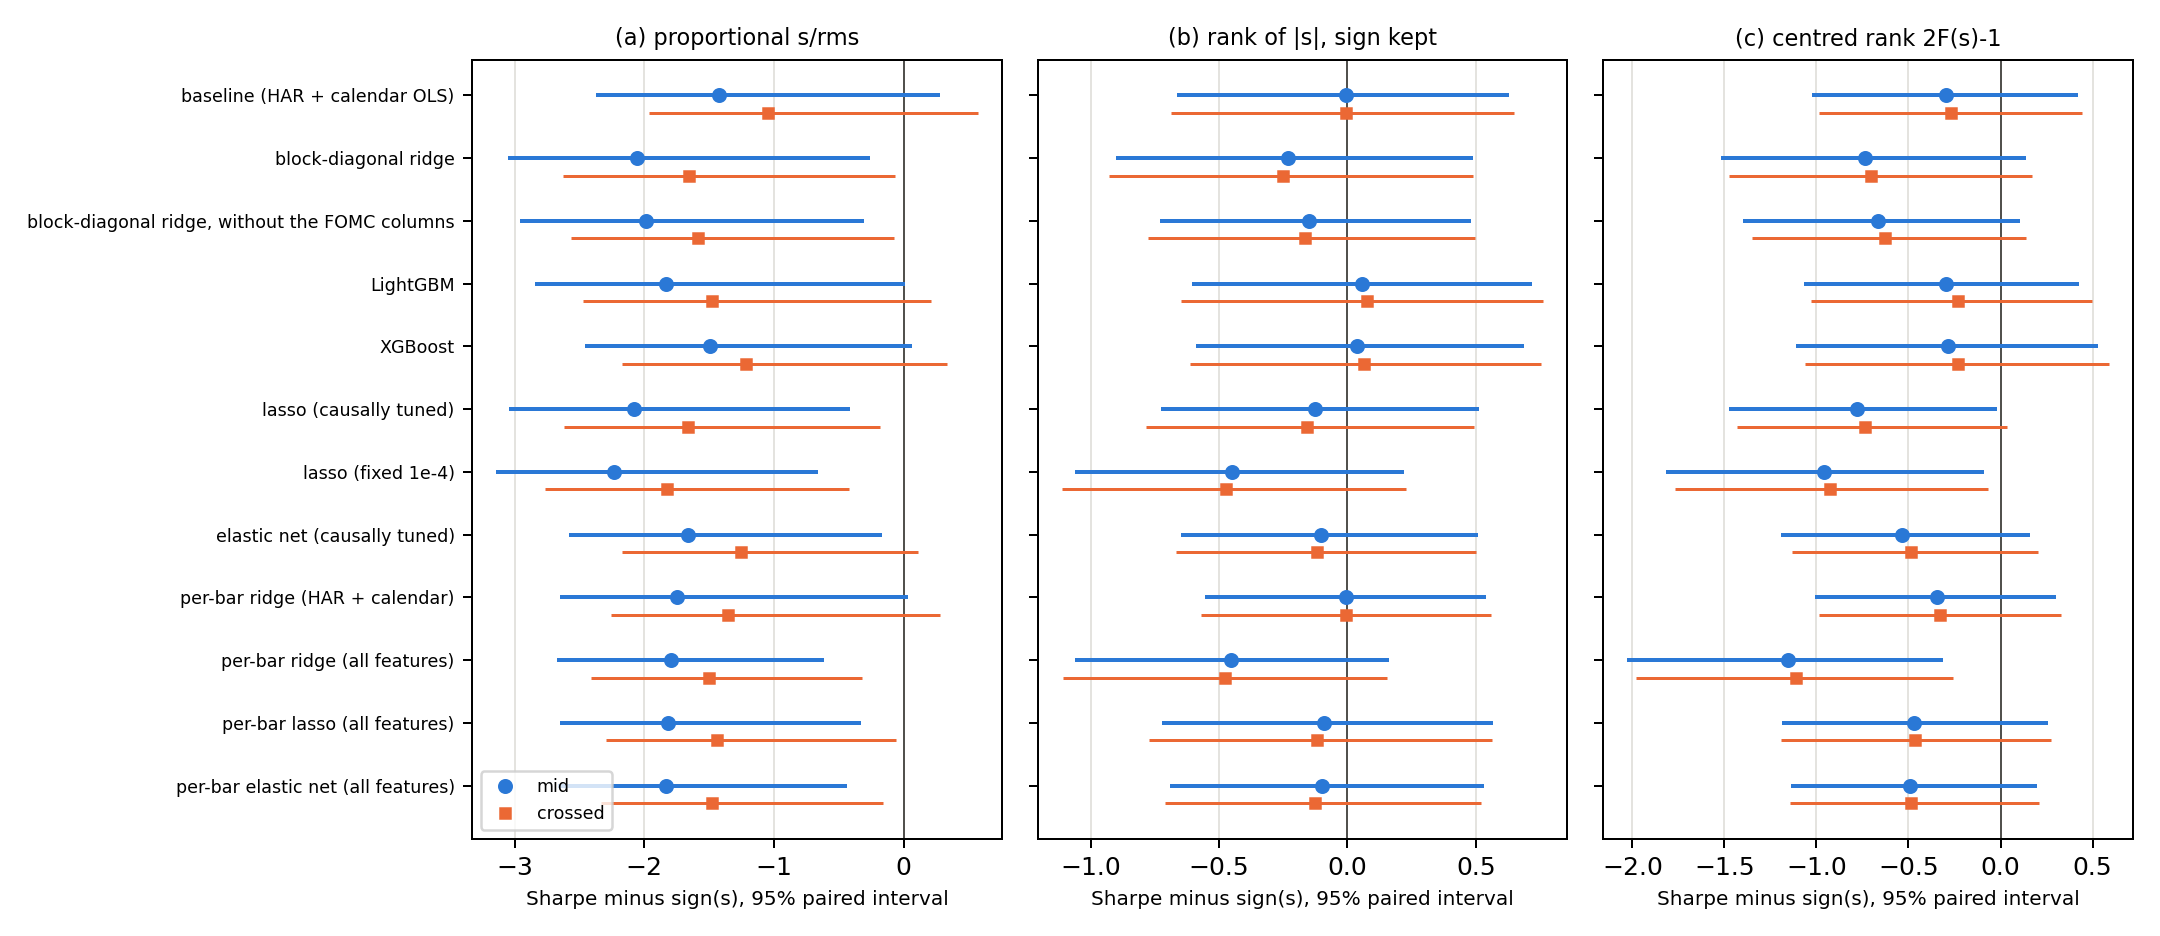
\includegraphics[width=0.9\linewidth]{../results/close_kelly/vrp_sizing_prop_rank.png}
\caption{Proportional and rank sizing: each rule's Sharpe minus sign(s)'s, per forecast, midpoint and crossed fills, with the paired 95\% interval (from the second day).}
\end{figure}
\begin{figure}[H]\centering
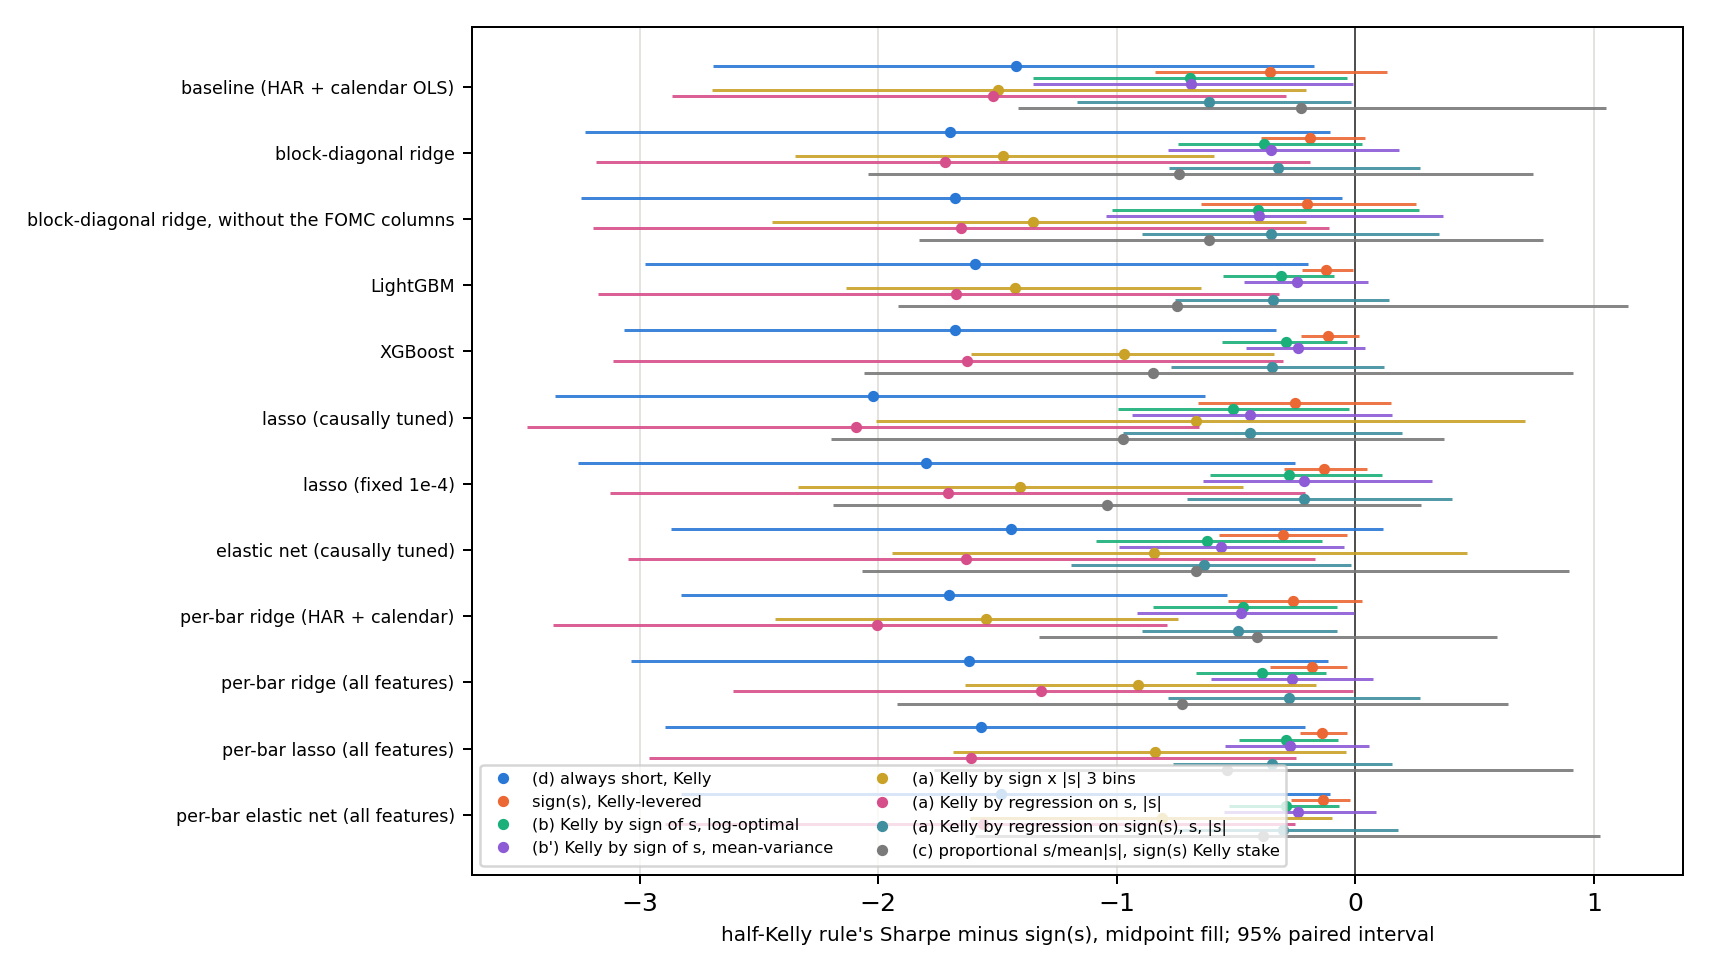
\includegraphics[width=0.9\linewidth]{../results/close_kelly/vrp_sizing_kelly_delta.png}
\caption{The Kelly family at half Kelly, midpoint fill: each rule's Sharpe minus sign(s)'s, per forecast, with the paired 95\% interval.}
\end{figure}
\begin{figure}[H]\centering
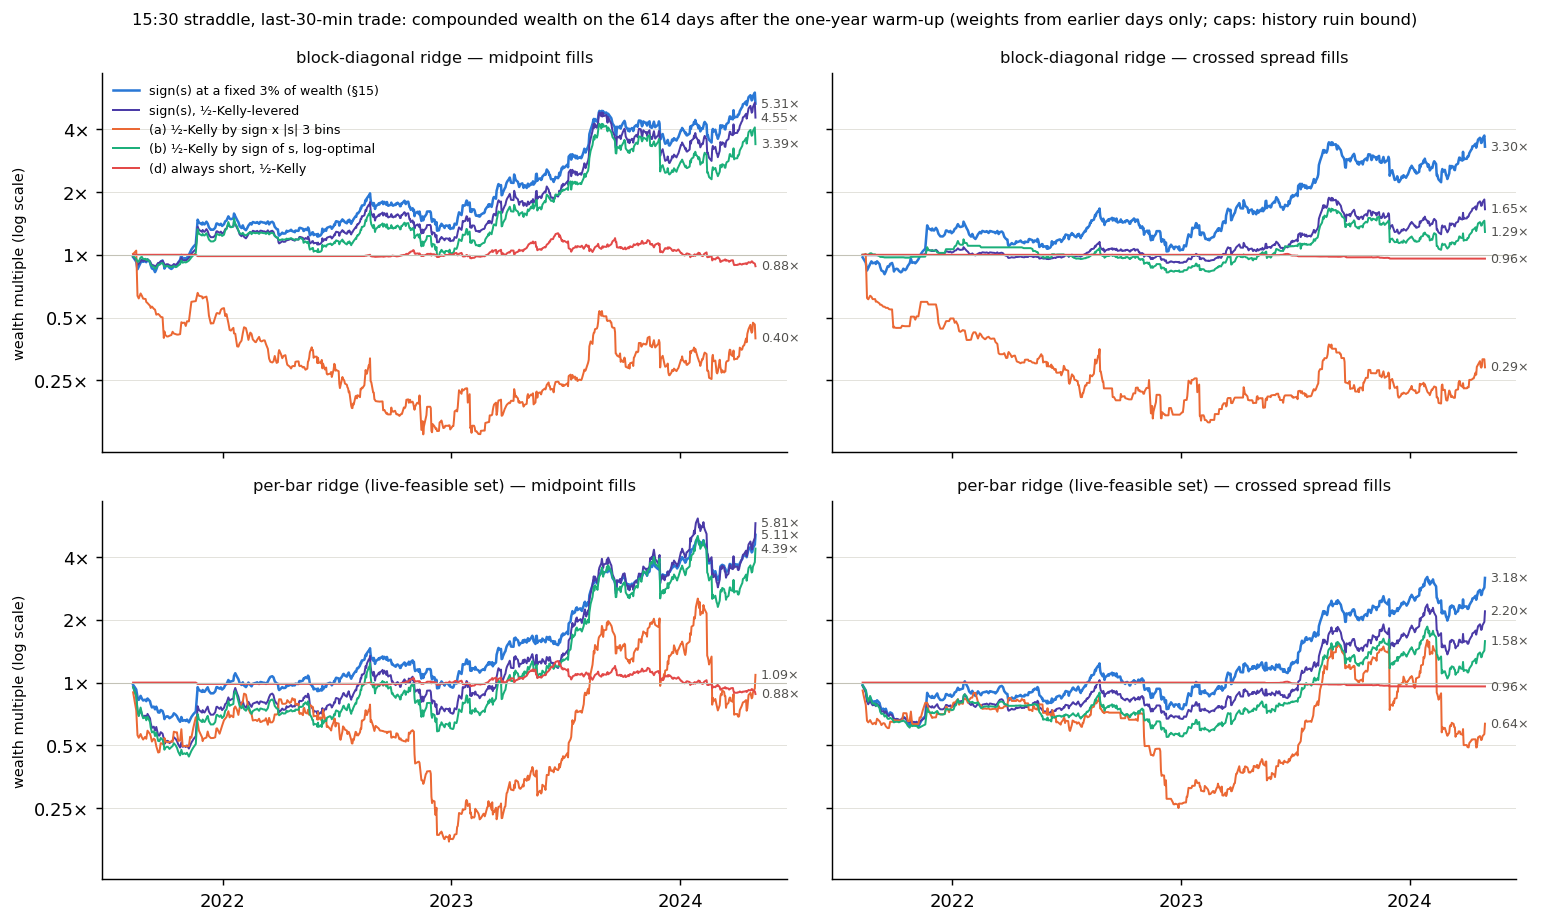
\includegraphics[width=0.9\linewidth]{../results/close_kelly/kelly_wealth.png}
\caption{Wealth paths (from experiments/close\_kelly\_sizing.py): sign(s) at a fixed 3\% of wealth, sign(s) Kelly-levered and always short.}
\end{figure}
\begin{figure}[H]\centering
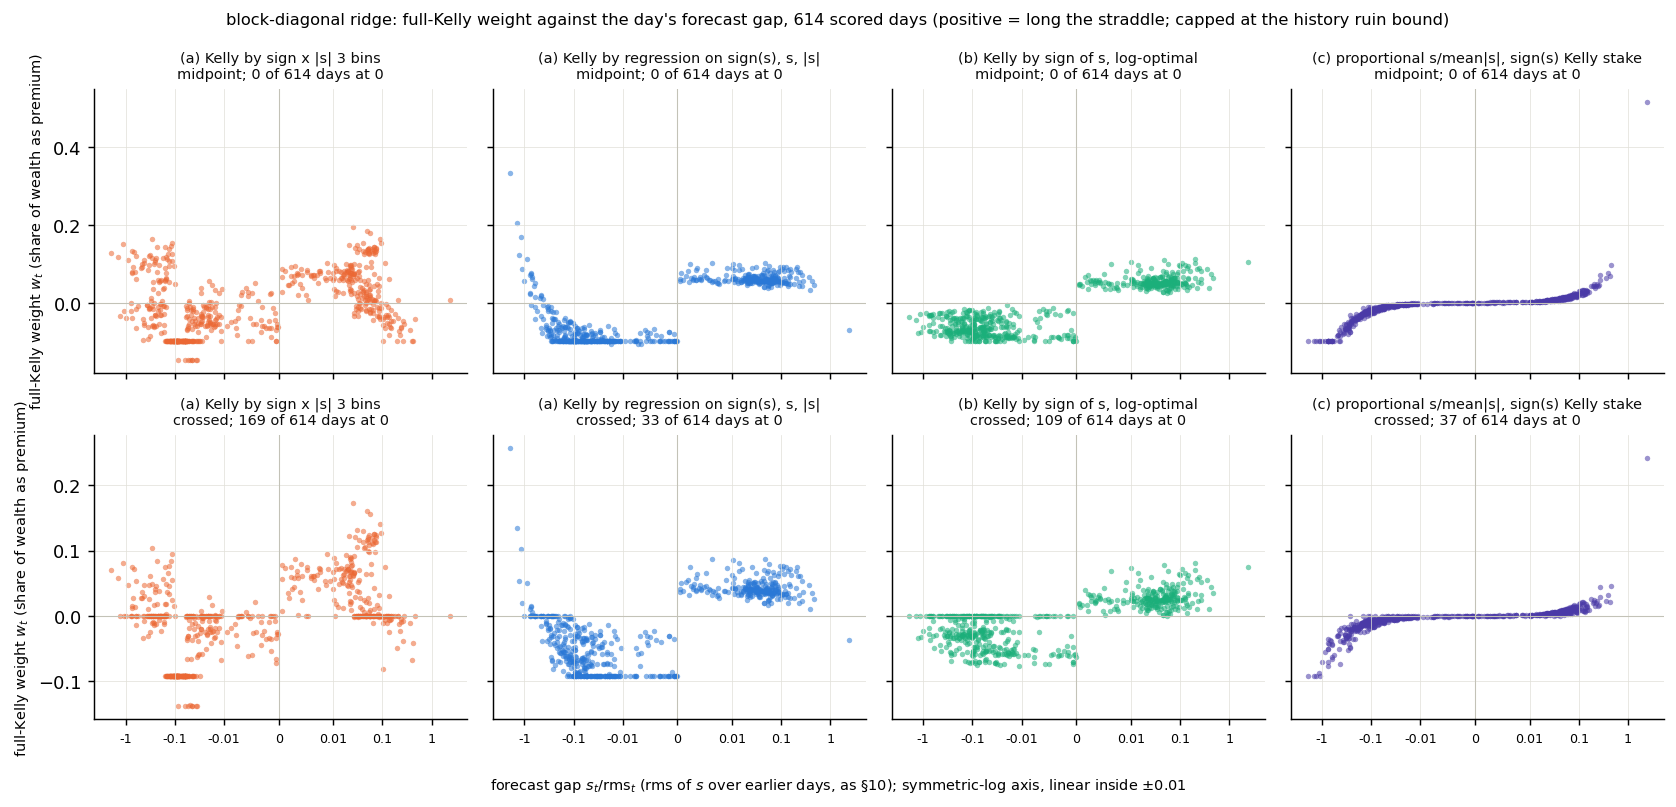
\includegraphics[width=0.9\linewidth]{../results/close_kelly/kelly_f_vs_s.png}
\caption{The Kelly fraction against the forecast gap $s_t$ (from experiments/close\_kelly\_sizing.py).}
\end{figure}
\end{document}
